\documentclass[11pt]{article}

\usepackage[a4paper,margin=27mm]{geometry}
\usepackage{fontspec}
\setmainfont{Latin Modern Roman}
\setsansfont{Latin Modern Sans}
\setmonofont{DejaVu Sans Mono}[Scale=MatchLowercase]
\usepackage{microtype}
\usepackage{amsmath,amssymb,amsthm,mathtools}
\numberwithin{equation}{section}
\usepackage{array}
\usepackage{booktabs}
\usepackage{enumitem}
\usepackage{float}
\usepackage{xcolor}
\usepackage{tikz}
\usetikzlibrary{arrows.meta,calc,decorations.pathreplacing,patterns,positioning,shapes.geometric}
\usepackage{pgfplots}
\pgfplotsset{compat=1.18}
\usepackage[hidelinks]{hyperref}
\setlength{\emergencystretch}{2em}
\hbadness=10000
\hfuzz=3pt

\newtheoremstyle{upright}
  {6pt}{6pt}{\normalfont}{}{\bfseries}{.}{.5em}{}
\theoremstyle{upright}
\newtheorem{theorem}{Theorem}[section]
\newtheorem{proposition}[theorem]{Proposition}
\newtheorem{corollary}[theorem]{Corollary}
\newtheorem{lemma}[theorem]{Lemma}
\theoremstyle{definition}
\newtheorem{definition}[theorem]{Definition}
\theoremstyle{remark}
\newtheorem{remark}[theorem]{Remark}

\newcommand{\F}{\mathbb F}
\newcommand{\PP}{\mathbb P}
\newcommand{\Tr}{\operatorname{Tr}}
\newcommand{\Span}{\operatorname{span}}
\newcommand{\LU}{\mathrm{LU}}
\newcommand{\LC}{\mathrm{LC}}
\newcommand{\AME}{\mathrm{AME}}
\newcommand{\GRS}{\mathrm{GRS}}
\newcommand{\supp}{\operatorname{supp}}
\newcommand{\rank}{\operatorname{rank}}
\newcommand{\diag}{\operatorname{diag}}
\newcolumntype{L}[1]{>{\raggedright\arraybackslash}p{#1}}

% These switches support anonymous one-figure-at-a-time comparisons of the
% exposition.  The committed paper includes every surviving figure.
\newcommand{\AMEFigureOne}{%
  \ifdefined\AMEHideFigureOne\else\begin{figure}[tbp]
\centering
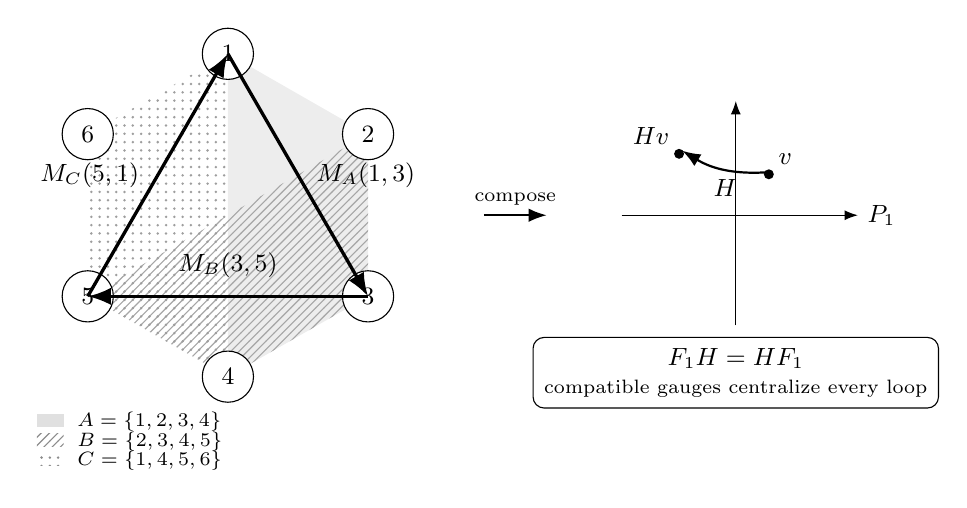
\begin{tikzpicture}[
  >=Latex,
  party/.style={circle,draw,fill=white,minimum size=6.5mm,inner sep=0pt,font=\small},
  push/.style={->,very thick},
  every node/.style={font=\small}
]
  \begin{scope}[xshift=-3.8cm]
    \coordinate (p1) at (0,2.05);
    \coordinate (p2) at (1.78,1.03);
    \coordinate (p3) at (1.78,-1.03);
    \coordinate (p4) at (0,-2.05);
    \coordinate (p5) at (-1.78,-1.03);
    \coordinate (p6) at (-1.78,1.03);

    % The three four-party supports used by the displayed loop.
    \fill[black!7] (p1) -- (p2) -- (p3) -- (p4) -- cycle;
    \fill[pattern=north east lines,pattern color=black!35]
      (p2) -- (p3) -- (p4) -- (p5) -- cycle;
    \fill[pattern=dots,pattern color=black!38]
      (p1) -- (p4) -- (p5) -- (p6) -- cycle;

    \foreach \n in {1,...,6} \node[party] at (p\n) {\n};
    \draw[push] (p1) -- node[right,xshift=1mm] {$M_A(1,3)$} (p3);
    \draw[push] (p3) -- node[above,yshift=1mm] {$M_B(3,5)$} (p5);
    \draw[push] (p5) -- node[left,xshift=-1mm] {$M_C(5,1)$} (p1);
    \node[align=left,anchor=north west,font=\scriptsize] at (-2.55,-2.38) {
      \tikz\fill[black!12] (0,0) rectangle (0.34,0.16);\; $A=\{1,2,3,4\}$\\[-1pt]
      \tikz\fill[pattern=north east lines,pattern color=black!45] (0,0) rectangle (0.34,0.16);\; $B=\{2,3,4,5\}$\\[-1pt]
      \tikz\fill[pattern=dots,pattern color=black!45] (0,0) rectangle (0.34,0.16);\; $C=\{1,4,5,6\}$
    };
  \end{scope}

  \draw[->,thick] (-0.55,0) -- (0.25,0)
    node[midway,above,font=\scriptsize] {compose};

  \begin{scope}[xshift=2.65cm]
    \draw[->] (-1.45,0) -- (1.55,0) node[right] {$P_1$};
    \draw[->] (0,-1.4) -- (0,1.45);
    \fill (0.42,0.52) circle (1.8pt) node[above right] {$v$};
    \fill (-0.72,0.78) circle (1.8pt) node[above left] {$Hv$};
    \draw[->,thick,bend left=18] (0.46,0.55) to
      node[below,font=\small] {$H$} (-0.68,0.82);
    \node[draw,rounded corners,align=center,inner sep=4pt] at (0,-2.0)
      {$F_1H=HF_1$\\[-1pt]
       \scriptsize compatible gauges centralize every loop};
  \end{scope}
\end{tikzpicture}
\caption{Operator pushing on minimum supports, shown for six parties.
Each \((m+1)\)-party support identifies the local Weyl-label planes of its
parties through the bijective projections of the support theorem; overlapping
supports compose to a loop whose holonomy \(H=M_CM_BM_A\) is a linear map of
the base plane, carrying a label \(v\) of the base plane to \(Hv\).
An atlas gauge is compatible precisely when it intertwines every transition;
for one state over a prime field, its base block centralizes every loop
holonomy.}
\label{fig:operator-holonomy}
\end{figure}
\fi}
\newcommand{\AMEFigureTwo}{%
  \ifdefined\AMEHideFigureTwo\else\begin{figure}[tbp]
\centering
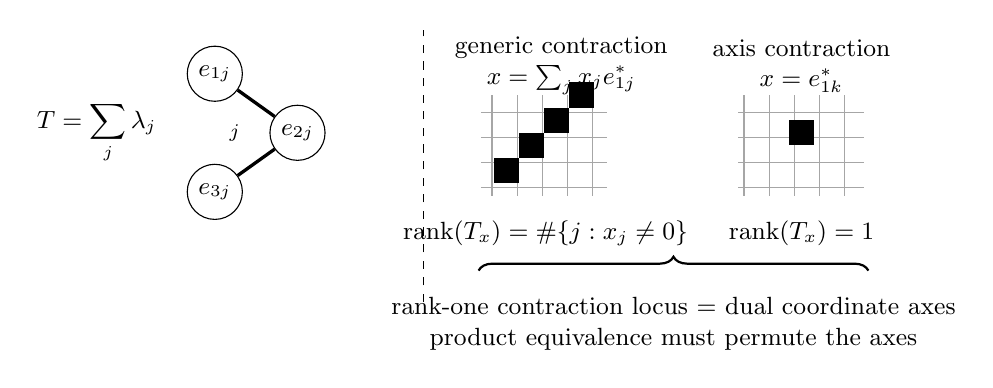
\begin{tikzpicture}[
  >=Latex,
  leg/.style={circle,draw,minimum size=7mm,inner sep=0pt},
  every node/.style={font=\small}
]
  \node (sum) at (-4.7,0.7) {$\displaystyle T=\sum_j\lambda_j$};
  \node[leg] (a) at (-3.2,1.45) {$e_{1j}$};
  \node[leg] (b) at (-2.15,0.7) {$e_{2j}$};
  \node[leg] (c) at (-3.2,-0.05) {$e_{3j}$};
  \draw[very thick] (a) -- (b) -- (c) -- cycle;
  \node[font=\scriptsize,fill=white,inner sep=1pt] at (-2.95,0.7) {$j$};

  \draw[dashed] (-0.55,-1.45) -- (-0.55,2.0);

  \node[align=center] at (1.2,1.55) {generic contraction\\$x=\sum_jx_je_{1j}^*$};
  \draw[step=0.32,black!35] (0.18,-0.1) grid (1.78,1.18);
  \foreach \x/\y in {0.34/0.06,0.66/0.38,0.98/0.70,1.30/1.02}
    \fill (\x,\y) rectangle ++(0.32,0.32);
  \node[align=center] at (1.0,-0.58)
    {$\rank(T_x)=\#\{j:x_j\ne0\}$};

  \node[align=center] at (4.25,1.55) {axis contraction\\$x=e_{1k}^*$};
  \draw[step=0.32,black!35] (3.45,-0.1) grid (5.05,1.18);
  \fill (4.09,0.54) rectangle ++(0.32,0.32);
  \node at (4.25,-0.58) {$\rank(T_x)=1$};

  \draw[decorate,decoration={brace,amplitude=5pt},thick]
    (0.15,-1.05) -- (5.1,-1.05)
    node[midway,below=6pt,align=center]
      {rank-one contraction locus $=$ dual coordinate axes\\
       product equivalence must permute the axes};
\end{tikzpicture}
\caption{A diagonal tensor with all coefficients nonzero exposes its own
axes.  Contracting one leg against \(x\) and flattening the remainder gives
rank equal to the number of nonzero coordinates of \(x\), so the rank-one
contraction locus is exactly the set of dual coordinate axes.  For an
\((m+1)\)-party AME marginal in local Hilbert--Schmidt spaces, the recovered
axes are the local Weyl axes, and a product conjugation must permute them.}
\label{fig:axis-recovery}
\end{figure}
\fi}
\newcommand{\AMEFigureFour}{%
  \ifdefined\AMEHideFigureFour\else
    Figure~\ref{fig:defect-landscape} gives a roadmap for the local estimates,
    the Clifford separation step, and the resulting explicit threshold.
    \begin{figure}[tbp]
\centering
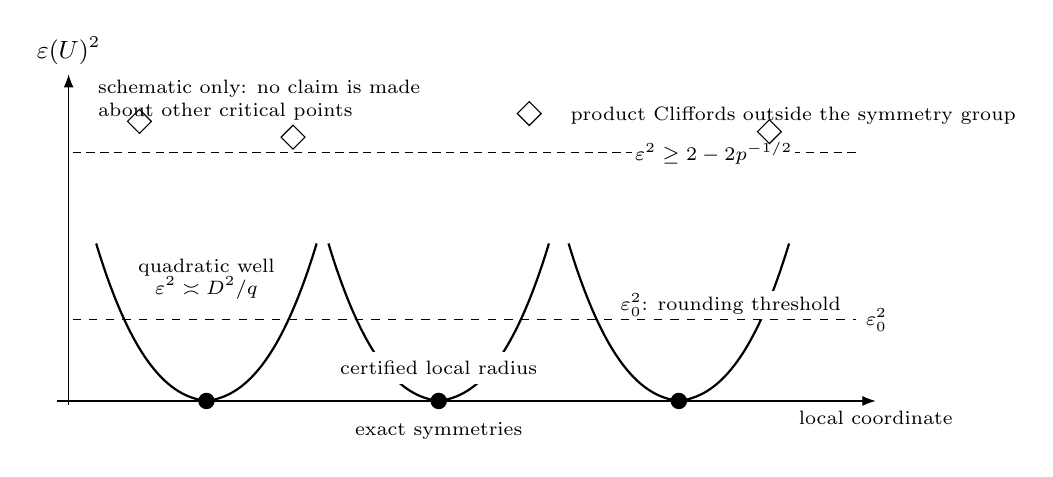
\begin{tikzpicture}[
  x=1cm,y=1cm,>=Latex,
  exact/.style={circle,fill=black,inner sep=2.1pt},
  clifford/.style={diamond,draw,fill=white,inner sep=2.2pt},
  every node/.style={font=\small}
]
  \draw[->] (-0.15,0) -- (10.25,0)
    node[right,below,font=\scriptsize] {local coordinate};
  \draw[->] (0,-0.05) -- (0,4.15) node[above] {$\varepsilon(U)^2$};

  \draw[thick]
    (0.35,2.0) .. controls (0.85,0.35) and (1.35,0.05) .. (1.75,0)
    .. controls (2.15,0.05) and (2.65,0.35) .. (3.15,2.0);
  \draw[thick]
    (3.3,2.0) .. controls (3.8,0.35) and (4.3,0.05) .. (4.7,0)
    .. controls (5.1,0.05) and (5.6,0.35) .. (6.1,2.0);
  \draw[thick]
    (6.35,2.0) .. controls (6.85,0.35) and (7.35,0.05) .. (7.75,0)
    .. controls (8.15,0.05) and (8.65,0.35) .. (9.15,2.0);

  \node[exact] at (1.75,0) {};
  \node[exact] at (4.7,0) {};
  \node[exact] at (7.75,0) {};
  \node[font=\scriptsize,anchor=north] at (4.7,-0.15)
    {exact symmetries};

  \draw[<->,thick] (3.85,0.42) -- (5.55,0.42);
  \node[fill=white,font=\scriptsize] at (4.7,0.42)
    {certified local radius};
  \node[font=\scriptsize,align=center] at (1.75,1.55)
    {quadratic well\\$\varepsilon^2\asymp D^2/q$};

  \draw[dashed] (0.05,1.03) -- (10.0,1.03)
    node[right,font=\scriptsize] {$\varepsilon_0^2$};
  \node[font=\scriptsize,anchor=south east,fill=white,inner sep=1pt]
    at (9.85,1.03) {$\varepsilon_0^2$: rounding threshold};

  \draw[densely dashed] (0.05,3.15) -- (10.0,3.15);
  \node[font=\scriptsize,align=left,anchor=west] at (6.25,3.62)
    {product Cliffords outside the symmetry group};
  \node[font=\scriptsize,anchor=west,fill=white,inner sep=1pt] at (7.15,3.15)
    {$\varepsilon^2\geq 2-2p^{-1/2}$};
  \foreach \x/\y in {0.9/3.55,2.85/3.35,5.85/3.65,8.9/3.42}
    \node[clifford] at (\x,\y) {};

  \node[font=\scriptsize,align=left,anchor=west] at (0.25,3.82)
    {schematic only: no claim is made\\about other critical points};
\end{tikzpicture}
\caption{Roadmap for the defect estimates (a one-dimensional schematic of a
high-dimensional product-unitary group).  Exact symmetries are isolated zeros
with certified local quadratic growth.  Every product Clifford outside the
symmetry group has defect at least \((2-2p^{-1/2})^{1/2}\); below the explicit
decomposition threshold, an arbitrary product unitary rounds to a Clifford and
then to an exact symmetry.  The picture asserts neither that every local
minimum is Clifford nor that the displayed coordinate exhausts the group.}
\label{fig:defect-landscape}
\end{figure}
%
  \fi}

\title{Robust Local-Unitary Rigidity of Stabilizer AME States}
\author{Tavis Rudd}
\date{August 2026}
\hypersetup{
  pdftitle={Robust Local-Unitary Rigidity of Stabilizer AME States},
  pdfauthor={Tavis Rudd}
}

\begin{document}
\maketitle

\begin{abstract}
Let \(q=p^e\) and \(m\geq2\).  We prove that every product unitary
mapping one stabilizer \(\AME(2m,q)\) state to another is Clifford on each
party, also when party relabelling is allowed.  The result covers arbitrary
additive stabilizers: local Clifford actions lie in
\(\operatorname{Sp}_{2e}(\F_p)\), with no \(\F_q\)-linearity assumption.
The proof is a support count.  Stabilizers contained in any
\((m+1)\)-party set project bijectively onto every retained party's Weyl
labels, so the reduced operator determines all local Weyl axes.

We also prove robust rigidity.  Below an explicit state-vector defect
threshold of order \(\min\{q^{-1/2},(2m)^{-1/2}\}\), a product unitary
decomposes into an exact symmetry and a residual whose collective generator
norm is at most \(\pi\sqrt q\,\varepsilon\).  Each local factor first
rounds to a Clifford within normalized Hilbert--Schmidt distance
\(8\varepsilon\).  Three-region cleaning and Weyl--Fourier concentration
give these frames; quantized stabilizer overlaps and a balanced-cut estimate
control the residual.

The exact proof also gives a complete finite transition-map invariant and
factorwise Clifford rigidity for transversal encoder conversions.
For promised stabilizer-AME check matrices, fixed-label recognition returns
compact symplectic witnesses in polynomial time in \(m\) for fixed \(q\);
stabilizer phases additionally determine a Clifford--Pauli conversion.
Selected marginal tests give fidelity certificates and an observable
sufficient condition for the robust theorem.
\end{abstract}
\noindent\textbf{Index Terms---}Absolutely maximally entangled states, local Clifford group, local-unitary
equivalence, minimum-support atlas, no-go theorems, quantitative rigidity,
quantum MDS codes, qudits, stabilizer cleaning, stabilizer codes,
symplectic group, transversal gates, Weyl operators.



\section{Introduction}

An absolutely maximally entangled state has maximally mixed reductions on
every set containing at most half of its parties.  Such states are also
called perfect tensors and, after one party is designated as an input, give
quantum maximum-distance-separable encoders.  They therefore sit at the
intersection of multipartite entanglement, stabilizer codes, transversal
gates, and tensor-network constructions.  Operationally, AME states serve as
resources for quantum error correction, threshold secret sharing, and
multi-user teleportation; a recent survey reviews these applications and
the known local-unitary classes \cite{RajchelMieldziocEtAl2026}.

This paper asks how rigid their local coordinates are.  With the party labels
fixed, two states are \emph{local-unitary (LU) equivalent} if a tensor product
of one-party unitaries maps one state ray to the other.  We say \emph{LU up to
party relabelling} when a party permutation is also allowed.  The analogous
relations are \emph{local-Clifford (LC) equivalence} and LC equivalence up to
party relabelling, with every one-party factor required to normalize the
chosen Weyl, or Pauli, system.  The theorem below uses the latter convention;
setting the permutation to the identity gives the fixed-label statement.
Local-Clifford equivalence is
discrete and can be studied through finite symplectic linear algebra;
local-unitary equivalence is a priori continuous and much larger.  The two
relations do not coincide for general stabilizer states
\cite{JiChenWeiYing2008}.

The distinction is both structural and operational.  LU equivalence asks
whether two preparations represent the same multipartite entanglement
resource after independent changes of local basis.  LC equivalence reduces
that question to finite symplectic data and is directly compatible with the
stabilizer description used for encoding and fault-tolerant gates.  For an
AME state viewed as an encoder Choi state, the same question asks whether a
transversal conversion can contain a genuinely non-Clifford factor.  A
quantitative version is needed when the conversion or symmetry is only
approximately realized.

Within the stabilizer AME class on an even number of at least four parties, maximal
entanglement removes that difference.

For \(q=p^e\), ``Clifford'' below always means the normalizer of the
additive Weyl system.  Its action on one-party labels lies in
\(\operatorname{Sp}_{2e}(\F_p)\); it need not be an \(\F_q\)-linear
\(2\times2\) transformation.

\begin{theorem}[Local-unitary rigidity]\label{thm:lu-lc-rigidity}
Let \(q=p^e\), let \(m\geq2\), and let
\(\lvert\psi\rangle,\lvert\phi\rangle\) be stabilizer
\(\AME(2m,q)\) states for the standard additive Weyl system.  Suppose
that, for a party permutation \(\pi\), single-qudit unitaries
\(U_1,\ldots,U_{2m}\), and a phase \(\theta\),
\[
 (U_1\otimes\cdots\otimes U_{2m})\pi\lvert\psi\rangle
   =e^{i\theta}\lvert\phi\rangle .
\]
Then every \(U_i\) normalizes the Weyl system.  Thus the displayed
equivalence is local Clifford.
\end{theorem}

The theorem converts a continuous equivalence problem into a finite one.
It is valid for every prime power, for arbitrary additive stabilizers, and
does not assume CSS form, equal stabilizer phases, classical linearity over
\(\F_q\), or a particular construction of the AME state.  The restriction
\(m\geq2\) is sharp: a Bell pair has the continuous symmetry
\(U\otimes\overline U\).

The proof uses one elementary support calculation.  On any \((m+1)\)-party
set, the stabilizer labels supported there form a group of order \(q^2\).
Projection onto the Weyl-label space \(\F_q^2\) of any retained party
is bijective; this space has dimension \(2e\) over \(\F_p\).  Consequently the reduced operator contains every local Weyl
axis exactly once in a matched diagonal decomposition.  The uniqueness of
that decomposition forces each local unitary to permute the Weyl axes and
hence to be Clifford.  In ordinary language,
\[
 \text{AME support counting}\ \Longrightarrow\
 \text{all local Weyl axes appear}\ \Longrightarrow\
 \text{every local factor is Clifford}.                 \tag{1.1}
\]

\subsection*{Quantitative question}

Exact rigidity does not by itself say what happens when a product unitary
only approximately preserves the state.  For
\(U=\bigotimes_iU_i\), define its state-vector defect by
\[
 \varepsilon(U)=\min_{|z|=1}
   \lVert U\lvert\psi\rangle-z\lvert\psi\rangle\rVert.
\]
The direct marginal proof is poorly conditioned for this problem: the
nonidentity part of one minimum-support marginal has exponentially small
Hilbert--Schmidt norm.  We instead regard each party in turn as the logical
leg of the associated \([[2m-1,1,m]]_q\) code.  Its physical parties can be
partitioned into three correctable regions.  A leakage-aware cleaning
argument tests the induced logical action by nested commutators, and a
finite Fourier argument rounds that action to a Clifford.

The exact constants are useful for applications, so we state them once in
the introduction.  Their scaling and proof mechanism are the main points.
Write \(G(\psi)\) for the group of product unitaries that preserve the ray
of \(\lvert\psi\rangle\).  We use the unnormalized Frobenius norm
\(\|h\|_F=(\Tr h^\dagger h)^{1/2}\); the normalized Hilbert--Schmidt
norm on one party is \(q^{-1/2}\|h\|_F\).

\begin{theorem}[Quantitative rounding]\label{thm:quantitative-rounding}
Let \(\lvert\psi\rangle\) be a stabilizer \(\AME(n,q)\) state with
\(n=2m\), \(m\geq2\), and let \(U=\bigotimes_iU_i\) be a product
unitary.  Put
\[
 R^{\mathrm{clean}}_{n,q}=
 \min\left\{\frac1{4\sqrt{2q}},\frac1{8\pi\sqrt n}\right\}.       \tag{1.2}
\]
If \(\varepsilon(U)<R^{\mathrm{clean}}_{n,q}\), then, up to phase,
\[
 U=g\bigotimes_{i=1}^n e^{ih_i},\qquad g\in G(\psi),
 \qquad
 \left(\sum_i\lVert h_i\rVert_F^2\right)^{1/2}
   \leq\pi\sqrt q\,\varepsilon(U),                     \tag{1.3}
\]
where the \(h_i\) are traceless Hermitian with spectral spread
\(\lambda_{\max}(h_i)-\lambda_{\min}(h_i)\) at most \(\pi\).  Before the
exact symmetry \(g\) is selected, each \(U_i\) is
within normalized Hilbert--Schmidt distance \(8\varepsilon(U)\) of a
one-qudit Clifford.  Uniformly over prime powers and existing AME states,
\[
 R^{\mathrm{clean}}_{n,q}
 =\Theta\!\left(\min\{q^{-1/2},n^{-1/2}\}\right).
\]
\end{theorem}

The proof has three stages.  First, quantitative cleaning places every
nested logical Weyl commutator within \(8\varepsilon\) of a scalar.
Second, Fourier concentration on the finite Weyl group produces a nearby
local Clifford at each party.  Third, the quantized overlap of stabilizer
states separates distinct product-Clifford branches by the uniform gap
\(d_p=(2-2p^{-1/2})^{1/2}\).  The AME second moment bounds the distance to the rounded Clifford branch;
a balanced-cut estimate using minimum-support labels then gives the
collective residual bound in \((1.3)\).  The radius is a
certified lower bound, not an optimality claim.

Here approximation refers to the state-vector defect of a product unitary
acting on an exact code state.  This differs from approximate
Eastin--Knill results, where error correction itself is relaxed; see, for
example, \cite{Alexander2025}.  The two questions share the same
fault-tolerance motivation but control different errors.

An exact product-unitary intertwiner between two states transfers this
result without changing the constants
(Corollary~\ref{cor:relative-intertwiner-rounding}).

The two headline proof branches are independent.  Support geometry first
recovers every Weyl axis, which yields exact rigidity and then the
transition-map and endomorphism structure.  Separately, the same support
geometry gives correctable regions, which feed the robust rounding theorem.
Appendix~\ref{sec:two-uniform} isolates the weaker consequences of pairwise
maximal mixing alone and is not used to prove either branch.

\subsection*{Consequences of the exact theorem}

The operational code consequence follows by treating one party as the
logical input of the associated quantum MDS encoder.  Throughout,
\emph{transversal} means a tensor product of one-site physical operators
with the physical coordinates fixed.  Such gates limit the direct spread
of errors between physical subsystems, which makes them central to
fault-tolerant constructions.  The Eastin--Knill theorem rules out a
universal transversal gate set for an exact finite-dimensional code
\cite{EastinKnill2009}; the natural family-specific question is therefore
which transversal gates remain.

\begin{corollary}[Factorwise transversal rigidity]
\label{cor:transversal-clifford}
Let \(m\geq2\), and let \(V_\psi,V_\phi:\mathbb C^q\to
(\mathbb C^q)^{\otimes(2m-1)}\) be encoders whose normalized Choi states
are stabilizer \(\AME(2m,q)\) states.  If \(U_i\in U(q)\) and
\[
 (U_1\otimes\cdots\otimes U_{2m-1})V_\psi=V_\phi L,
\]
then \(L\) and every \(U_i\) are Clifford.  In particular, no code in
this family admits a transversal non-Clifford logical unitary.
\end{corollary}

General cleaning arguments already constrain the \emph{logical} action of
a transversal gate \cite[Lemma~5]{PastawskiYoshida2015}.
Corollary~\ref{cor:transversal-clifford} is stronger in
a different direction: it identifies every physical one-site factor as
Clifford as well as the induced logical gate.  This factorwise conclusion
is what turns LU equivalence of the Choi states into finite local
symplectic data.

\paragraph{Transition maps.}

The support bijections retain how the local Weyl frames are related.  For an
\((m+1)\)-party support \(A\), projection at party \(i\) gives a bijection
\(p_i:L_\psi(A)\to\F_q^2\).  The maps
\[
 M_A(i,j)=p_jp_i^{-1}
\]
are the usual operator-pushing maps between the local Weyl-label spaces.
Their compositions around closed paths are holonomies.

\begin{theorem}[Classification by minimum-support transition maps]
\label{thm:atlas-classification}
Let \(m\geq2\).  After a fixed party relabelling, two stabilizer
\(\AME(2m,q)\) states are LU equivalent exactly when their systems of
minimum-support transition maps
are equivalent by local trace-symplectic changes of Weyl frame.  For one
state, if \(\operatorname{Aut}_{\mathrm{tr}}(\psi)\) is the group of
compatible local symplectic automorphisms of the transition system and
\(\Gamma_\psi\) its fixed-party projective
product-unitary symmetry group, then
\[
 1\longrightarrow L_\psi\longrightarrow\Gamma_\psi
  \longrightarrow\operatorname{Aut}_{\mathrm{tr}}(\psi)\longrightarrow1
\]
is exact.  When \(q\) is prime, \(\operatorname{Aut}_{\mathrm{tr}}(\psi)\)
is the determinant-one unit group of the local endomorphism algebra described
in Section~\ref{sec:endomorphism-algebra}.
\end{theorem}

The invariant is also effective.  After fixing any half-set of parties,
only the \(m\) minimum supports obtained by adjoining one complementary
party are needed: their supported label groups form a direct sum equal to
the full stabilizer label space, and no smaller collection of
minimum-support subgroups can span it
(Proposition~\ref{prop:half-set-direct-sum}).  Fixed-label recognition then
enumerates one base symplectic frame and checks each candidate by finite
linear algebra.  In particular, it is polynomial in \(m\) for fixed local
dimension.  Corollary~\ref{cor:finite-recognition} gives the explicit
candidate count and the separate cost of unknown party relabelling.
The input is promised stabilizer-AME check matrices with fixed party labels;
the output is a compact symplectic witness, upgraded to a Clifford--Pauli
conversion when stabilizer phases are supplied.  These data also determine
an intrinsic endomorphism algebra in prime dimension
(Section~\ref{sec:endomorphism-algebra}), certify the state from \(m\)
minimum-support marginals, and decide stochastic local conversion
(Sections~\ref{subsec:marginal-certification} and~\ref{subsec:stochastic-conversion}).  Complementary marginal tests also give a fidelity certificate with gap
\((m+1)/(2m)\), supplying an observable sufficient condition for robust
rigidity when the preparation is promised to be a product-unitary image
(Section~\ref{subsec:optimal-marginal-verification}).  These consequences
are optional on a first reading of the two rigidity proofs.

At the radius
\[
 R^{\mathrm{trans}}=\frac{\sqrt2}{68},                 \tag{1.4}
\]
independent of both party count and local dimension,
the symplectic maps recovered by cleaning already preserve every transition
map exactly.  This does not yet identify the exact product symmetry.
Localized commutators cancel Weyl-translation phases, so they determine the
stabilizer label space but not its character.  The resulting product-Pauli
correction need not be close to the rounded product Clifford.  We refer to
this as the unresolved stabilizer-character, or product-Pauli phase,
correction.  Controlling it is the missing ingredient in a
party-count-independent global entry radius.

\subsection*{Relation to prior work and contribution}

The exact three-cleanable-region Clifford obstruction is due to Pastawski
and Yoshida \cite[Lemma~5]{PastawskiYoshida2015}, building on stabilizer
cleaning \cite[Lemma~1]{BravyiTerhal2009} and the localization method behind
transversal-gate hierarchy bounds
\cite{BravyiKonig2013,JochymOConnorKubicaYoder2018}.  We use only the exact
cleaning and localization consequences and prove the leakage estimate,
finite Weyl--Fourier rounding, and explicit AME composition here.

For exact LU rigidity, Rains recovered the three Pauli axes from a diagonal
correlation tensor, and Van den Nest, Dehaene, and De Moor used that mechanism
in a minimum-support criterion for qubit stabilizer states
\cite[Theorem~13]{Rains1999}
\cite[Theorem~1 and Corollary~1]{VanDenNestDehaeneDeMoor2005}.
Under their qubit minimum-support hypotheses, their proof already makes
the factors of the given LU Clifford.  Our extension is the automatic
complete-Weyl-support condition for arbitrary additive prime-power AME
states, together with the constructive and quantitative conclusions.
Subsequent work developed further sufficient conditions and exposed the
limits of the LU--LC conjecture
\cite{ZengChungCrossChuang2007,GrossVanDenNest2008,JiChenWeiYing2008}.
Englbrecht and Kraus classify all qubit stabilizer local symmetries
\cite{EnglbrechtKraus2020}.  More recently, Claudet and Perdrix gave a
graphical characterization using generalized local complementation and a
quasi-polynomial decision algorithm, while Burchardt, de Jong, and Vandr\'e
reduced verification to modular linear equations
\cite{ClaudetPerdrix2024,ClaudetPerdrix2025Algorithm,
BurchardtDeJongVandre2024}.  The general qubit problem is now sharply
separated from the AME case: LU and LC agree through 26 qubits but already
differ at 27 \cite{Claudet2026Minimal}.  The present support argument
instead uses the AME condition to extend the axis-recovery mechanism to
arbitrary additive prime-power stabilizers.  Because every minimum support
contains the full local Weyl basis, no additional minimum-support
hypothesis is required.

Tan proves the general AME--quantum-MDS orbit and
symmetry--transversal correspondences \cite[Theorems~3.5 and~3.6]{Tan2026}
and computes the four-qutrit symmetry and transversal groups
\cite[Theorem~5.3]{Tan2026}; separate work classifies five-qubit AME states
\cite{TanFiveQubit2026}.  To our knowledge, the missing
uniform statement was that every factor in an arbitrary additive
prime-power stabilizer-AME conversion is Clifford, at every even length for
which such a state exists.  Our exact result supplies that factorwise
statement, a complete transition-map invariant, and the finite recognition
bound above.  The same half-set geometry shows that \(m\) reductions to
\(m+1\) parties determine the state among all density operators, with both
numbers optimal and an explicit parent Hamiltonian, and that the unitarity
hypothesis can be dropped: every invertible product operator between two
such states is Clifford up to scalars
(Sections~\ref{subsec:marginal-certification} and~\ref{subsec:stochastic-conversion}).  The first statement
sharpens the generator-support criterion for qubit stabilizer states
\cite[Theorem~2]{WuYangWangWenQin2015}; the second strengthens the
Kempf--Ness equality of SLOCC and LU classes for AME states
\cite[Corollary~1]{BurchardtRaissi2020}.
The exact result also identifies, in prime dimension, the intrinsic
endomorphism algebra behind the symmetry calculation.  To our knowledge, no
earlier result forces this algebra to be nonscalar for every four- or
six-party stabilizer AME state; Tan's four-qutrit computation is an important
special case.  The
quantitative result supplies an explicit neighborhood in which an
approximate product symmetry can be assigned to an exact Clifford branch,
while distinguishing symplectic compatibility from the remaining
stabilizer-character correction.  No new qualitative
transversal-hierarchy obstruction is claimed.

The class continues to acquire nontrivial examples: recent self-dual MDS
constructions establish stabilizer \(\AME(12,5)\), \(\AME(18,11)\), and
\(\AME(18,13)\) states \cite{BevinsBidav2026}.  Our results apply to such
states without selecting a CSS, graph-state, or \(\F_q\)-linear
presentation.  Recent work classifies diagonal transversal Clifford groups
and characterizes code-preserving Clifford circuits for broader binary code
families and circuit models \cite{DasuBurton2025,Albert2026}; here the input
is instead the maximal entanglement of one stabilizer state, and the
conclusion begins with an arbitrary product unitary.

The stabilizer assumption is essential to the discrete transition system.
General AME families can contain infinitely many LU classes; Ramadas and
Lakshminarayan give an orthogonal-array criterion producing such families
\cite[Theorem~1 and Corollary~1]{RamadasLakshminarayan2025}.  Perfect-tensor
operator pushing and the encoder interpretation are used explicitly in
holographic codes \cite[Eq.~(2.3) and Section~5.7]{PastawskiYoshidaHarlowPreskill2015}.

\subsection*{Reading the paper}

For the two main results, read the support dictionary in
Section~\ref{sec:dictionary}, the exact proof in
Section~\ref{sec:rigidity}, and the robust proof in
Section~\ref{sec:quantitative}.  The four-qutrit example in
Section~\ref{subsec:four-qutrit-example} makes the support, frame and
character data explicit.  Its marginal tests in
Section~\ref{subsec:optimal-marginal-verification} lead to the observable
rounding criterion in Corollary~\ref{cor:marginal-certified-rounding}.

The finite classification and encoder consequences occupy the rest of
Section~\ref{sec:atlas}; Section~\ref{sec:endomorphism-algebra} refines
the classification in prime dimension.  The robust proof uses the Pauli-compatible Choi encoder from
Section~\ref{subsec:encoder-consequences}; its transition-map refinement
also uses the atlas and character repair in Section~\ref{sec:atlas}.
The remaining classification material is optional on the first route.  The appendices give the associated code structures,
stabilizer-independent infinitesimal estimates, weighted and nonstabilizer
marginal-test refinements, and the formal trust boundary.  They are not
needed for either headline rigidity theorem.

\section{From six-arcs to AME tensors}

This section will fix the projective, code-equivalence, stabilizer, and
party-permutation conventions.  It will state the six-arc/MDS/CSS/AME
dictionary used by every later theorem and identify the degenerate and
$\GRS$ boundary loci.

\section{Complete Weyl-basis marginals and LU rigidity}\label{sec:rigidity}

We first isolate the linear-algebra statement that recovers a diagonal
tensor's coordinate axes.  It is the complete-Weyl-basis counterpart of the
three-Pauli argument in \cite{Rains1999,VanDenNestDehaeneDeMoor2005}.
The statement itself is classical: it is Jennrich's uniqueness theorem for
trilinear decompositions, published in \cite[\S V]{Harshman1970} and there
credited to Jennrich, whose conclusion that the factor matrices agree up to
one permutation and compensating diagonal scalings is the monomial property
below.  It is the full-column-rank case of Kruskal's condition
\cite{Kruskal1977}, extended to arbitrarily many factors in
\cite{SidiropoulosBro2000}; see \cite[\S3.2]{KoldaBader2009} for the
attribution and for a survey of the uniqueness theory.  We give a short
self-contained proof because the contraction argument is the one used in
Proposition~\ref{prop:full-weyl-marginal}, and claim no novelty for either
the statement or the proof.

\begin{lemma}[Diagonal-tensor axes]\label{lem:diagonal-axes}
Let \(r\geq3\), let \(E_1,\ldots,E_r\) be \(N\)-dimensional complex inner
product spaces, and choose orthonormal bases
\(\{e_{ij}:1\leq j\leq N\}\).  If
\[
 T=\sum_{j=1}^N\lambda_j
 e_{1j}\otimes\cdots\otimes e_{rj},\qquad \lambda_j\ne0,       \tag{3.1}
\]
then the coordinate axes in every \(E_i\) are intrinsic to \(T\).
Consequently, a product of invertible linear maps carrying one tensor of
the form \((3.1)\) to another is monomial in the displayed bases.
\end{lemma}

\begin{proof}
For nonzero \(x=\sum_jx_je_{1j}^*\), contract the first factor against
\(x\).  The result is
\[
 T_x=\sum_j\lambda_jx_j e_{2j}\otimes\cdots\otimes e_{rj}.
\]
Flattening from \(E_2\) to \(E_3\otimes\cdots\otimes E_r\) gives a matrix
of rank \(\#\{j:x_j\ne0\}\).  Thus \(T_x\) has rank one exactly when
the ray of \(x\) is a dual coordinate axis.  Product equivalence preserves
this projective rank-one contraction locus.  The inner products identify
the recovered dual axes with the coordinate axes in the first factor.
Apply the same argument in every factor.
\end{proof}

\AMEFigureTwo

To avoid repeatedly stating the matched-basis condition, call an operator on
\(r\geq3\) qudits \emph{Weyl-diagonal with complete local support} if there
is a \(q^2\)-element set \(P\), a distinguished element \(0\in P\), and
bijections \(f_i:P\to\F_q^2\) with \(f_i(0)=0\), for which
\[
 R=\sum_{v\in P}\lambda_v
       \bigotimes_{i=1}^r W_{f_i(v)},\qquad \lambda_v\ne0.       \tag{3.2}
\]
The coefficients need not be equal.  What matters is that the same
\(q^2\)-element index set runs bijectively through the complete local
Weyl basis at every party.  Neither \(P\) nor the bijections need be
\(\F_q\)-linear.

\begin{proposition}[Complete Weyl-basis marginal criterion]
\label{prop:full-weyl-marginal}
Let \(R\) and \(R'\) be Weyl-diagonal operators with complete local support
on the same
\(r\geq3\) parties, possibly with different indexing sets, bijections,
and coefficients.  If
\[
 R'=(U_1\otimes\cdots\otimes U_r)R
       (U_1\otimes\cdots\otimes U_r)^\dagger ,
\]
then every \(U_i\) is Clifford.
\end{proposition}

\begin{proof}
View \(R\) and \(R'\) as tensors in the local Hilbert--Schmidt spaces.
After replacing \(W_v\) by the orthonormal basis \(q^{-1/2}W_v\) and
absorbing the common normalization into the coefficients, both have the
form in Lemma~\ref{lem:diagonal-axes}, with \(N=q^2\).
Local conjugation acts invertibly on each factor, so it must permute the
Weyl axes.  It fixes the identity operator and hence the identity axis.
It therefore permutes the nonidentity projective Weyl operators, which
is exactly the single-qudit Clifford condition.
\end{proof}

\begin{corollary}[Marginal-cover rigidity]
\label{cor:full-weyl-cover}
Let \(\lvert\psi\rangle,\lvert\phi\rangle\) be \(n\)-qudit states and
suppose a product unitary carries \(\lvert\psi\rangle\) to
\(\lvert\phi\rangle\) up to phase, any party permutation having first been
absorbed by relabelling \(\lvert\phi\rangle\), so that the two states are
indexed by the same parties.  If every
party belongs to a set \(S\) of at least three parties for which both
reduced operators \(\rho^\psi_S\) and \(\rho^\phi_S\) are Weyl-diagonal
with complete local support, then every local factor is Clifford.
\end{corollary}

\begin{proof}
Partial trace gives a product-unitary equivalence of the two reduced
operators on each chosen \(S\).  Apply
Proposition~\ref{prop:full-weyl-marginal}; the chosen sets cover all
parties.
\end{proof}

\begin{proposition}[Stabilizer-AME support theorem]
\label{prop:stabilizer-ame-support}
Let \(\lvert\psi\rangle\) be a stabilizer
\(\AME(2m,q)\) state, and let \(A\) be any \(m+1\) parties.  Then
\[
 |L(A)|=q^2.
\]
Every nonidentity label in \(L(A)\) has support exactly \(A\), and for
each \(i\in A\) the coordinate projection
\[
 p_i:L(A)\longrightarrow\F_q^2
\]
is bijective.
\end{proposition}

\begin{proof}
The projective label group \(L\) has order \(q^{2m}\).  Restrict its
labels to the \(m-1\) parties outside \(A\).  The target has order
\(q^{2(m-1)}\), and the kernel is \(L(A)\); hence
\[
 |L(A)|\geq q^{2m}/q^{2(m-1)}=q^2.                    \tag{3.3}
\]
Fix \(i\in A\).  A label in the kernel of \(p_i\) is supported on the
\(m\)-set \(A\setminus\{i\}\).  The AME condition and \((2.3)\) exclude
every such nonidentity stabilizer, so \(p_i\) is injective.  Its codomain
has order \(q^2\), giving the reverse inequality in \((3.3)\) and hence
bijectivity.  The same no-small-support argument shows that every
nonidentity element of \(L(A)\) has full support \(A\).
\end{proof}

\begin{proposition}[A stabilizer-AME marginal fixes the local Weyl axes]
\label{prop:marginal-axes}
Let \(\lvert\psi\rangle,\lvert\phi\rangle\) be stabilizer
\(\AME(2m,q)\) states.  If a product unitary on an \((m+1)\)-set \(A\)
carries \(\rho^\psi_A\) to \(\rho^\phi_A\), then every local factor on
\(A\) is Clifford.
\end{proposition}

\begin{proof}
By \((2.3)\),
\[
 \rho^\psi_A=q^{-|A|}
   \sum_{\ell\in L_\psi(A)}\widetilde W_\ell .
\]
Index this sum by \(P=L_\psi(A)\).  Proposition
\ref{prop:stabilizer-ame-support} says that every coordinate projection
\(P\to\F_q^2\) is bijective.  Relative to the fixed Weyl convention, each
stabilizer lift contributes a nonzero coefficient.  Thus
\(\rho^\psi_A\) is Weyl-diagonal with complete local support in the sense of
\((3.2)\), and the same holds for \(\rho^\phi_A\).  Apply
Proposition~\ref{prop:full-weyl-marginal}.
\end{proof}

\begin{proof}[Proof of Theorem~\ref{thm:lu-lc-rigidity}]
Absorb the party permutation by relabelling \(\lvert\phi\rangle\).  Partial
trace gives a product-unitary equivalence
\(\rho^\psi_A\sim\rho^\phi_A\) for every \((m+1)\)-set \(A\).  Given a
party \(i\), choose such a set containing it and apply
Proposition~\ref{prop:marginal-axes}.  Thus every \(U_i\) is Clifford.
\end{proof}

\section{Minimum-support transition maps and encoder consequences}
\label{sec:atlas}

The same support calculation recovers standard quantum-MDS structure.
If \(|A|\leq m\), the AME condition gives \(L(A)=\{0\}\).  If
\(|A|>m\), then \(\rho^\psi_{A^c}\) is maximally mixed, so purity of the
global state gives
\(\Tr((\rho^\psi_A)^2)=q^{-(2m-|A|)}\).  On the other hand, \((2.3)\)
and Weyl orthogonality give
\(\Tr((\rho^\psi_A)^2)=q^{-|A|}|L(A)|\).  Hence, for every party set
\(A\),
\[
 |L(A)|=q^{2\max(|A|-m,0)}.                              \tag{4.1}
\]
M\"obius inversion is the stabilizer-state specialization of the
quantum-MDS Shor--Laflamme distribution of Huber and Grassl
\cite[Theorems~8 and 9]{HuberGrassl2020}; in particular the number of
weight-\(m+1\) projective stabilizers is
\(\binom{2m}{m+1}(q^2-1)\).  The following systematic form strengthens
minimum-weight generation: recognition needs only \(m\) of these supports,
and that number is optimal among spanning families of minimum-support
subgroups.

\begin{proposition}[Half-set systematic decomposition]
\label{prop:half-set-direct-sum}
Fix an \(m\)-party set \(B\), and let \(P_j=\F_q^2\) be the local label
space at party \(j\).  The coordinate projection
\[
 \operatorname{pr}_{B^c}:L\longrightarrow
 \bigoplus_{j\notin B}P_j
\]
is an isomorphism of additive groups.  Hence there is a unique
\(\F_p\)-linear map
\[
 K_B:\bigoplus_{j\notin B}P_j\longrightarrow
     \bigoplus_{i\in B}P_i
\]
whose graph is \(L\).  For the direct-sum trace-symplectic forms it
satisfies
\[
 [K_Bx,K_By]_B=-[x,y]_{B^c}.
\]
After local \(\F_p\)-bases are chosen, row reduction therefore puts any
row-generator check matrix for \(L\), ordered as \(B,B^c\), in systematic
form \([K_B^{\mathsf T}\mid I]\); here \(K_B\) acts on column vectors.
Moreover, if \(I\subseteq B\), \(J\subseteq B^c\), and
\(|I|=|J|\), then the party-block submatrix
\[
 K_{I,J}:\bigoplus_{j\in J}P_j\longrightarrow
          \bigoplus_{i\in I}P_i
\]
is an isomorphism.
Conversely, a maximal isotropic subspace of the form
\(\operatorname{graph}(K_B)\) is the label space of a stabilizer AME state
exactly when all these party-aligned square block maps are isomorphisms.
Moreover, \(K_{I,J}\) is invertible if and only if the complementary block
\(K_{B\setminus I,B^c\setminus J}\) is invertible.  Thus it suffices to test
one representative of each complementary pair.

For each \(j\notin B\), put
\(A_j=B\cup\{j\}\).  The inverse image of the \(j\)-th coordinate
summand is \(L(A_j)\), and therefore
\[
 L=\bigoplus_{j\notin B}L(A_j).
\]
Thus these \(m\) minimum-support subgroups determine the full stabilizer
label group.  Moreover, no collection of fewer than \(m\)
minimum-support subgroups can span \(L\).
\end{proposition}

\begin{proof}
The kernel of \(\operatorname{pr}_{B^c}\) is \(L(B)=\{0\}\) by the AME
support condition.  Its domain and codomain both have order \(q^{2m}\),
so it is an isomorphism.  This gives the graph map \(K_B\) and the
systematic check-matrix form.  Since \(L\) is isotropic, evaluating the
ambient direct-sum symplectic form on \((K_Bx,x)\) and \((K_By,y)\) gives
the displayed identity.

For the block statement, let
\(S=I\cup(B^c\setminus J)\), so \(|S|=m\).  Projection \(L\to
\bigoplus_{s\in S}P_s\) is an isomorphism by the same kernel-and-order
argument.  If \(x\) is supported on \(J\) and \(K_{I,J}x=0\), then
\((K_Bx,x)\in L\) projects to zero on \(S\).  Thus \(x=0\).
The source and target of \(K_{I,J}\) have equal dimension, so the block
map is an isomorphism.

Conversely, every \(m\)-party set has the form
\(I\cup(B^c\setminus J)\) with \(|I|=|J|\).  The kernel of projection
from \(\operatorname{graph}(K_B)\) to this set is naturally
\(\ker K_{I,J}\).  If all the displayed block maps are isomorphisms, every
half-set projection is therefore injective and hence bijective.  Equivalently,
there is no nonzero stabilizer label supported on at most \(m\) parties,
which is the stabilizer AME condition.

For complementarity, \(K_{I,J}\) is invertible exactly when
\(K_B(\bigoplus_{j\in J}P_j)\) is transverse to
\(\bigoplus_{i\in B\setminus I}P_i\).  Taking symplectic orthogonal
complements and using the anti-symplectic identity for \(K_B\) gives the
same condition for \(K_{B\setminus I,B^c\setminus J}\).

The inverse image of the \(j\)-th coordinate
summand consists exactly of the labels supported on \(B\cup\{j\}\).
Pulling back the coordinate direct sum gives the displayed decomposition.

Every minimum-support subgroup has order \(q^2\) by
Proposition~\ref{prop:stabilizer-ame-support}.  A sum of \(r\) such
subgroups has order at most \(q^{2r}\), whereas \(|L|=q^{2m}\).
Spanning \(L\) therefore requires \(r\geq m\).
\end{proof}

We now prove the transition-map classification stated in the introduction.
Regard each local label group
\[
 P_i=\F_q^2
\]
as a \(2e\)-dimensional trace-symplectic space over \(\F_p\).  For every
\((m+1)\)-set \(A\) and \(i,j\in A\), the support theorem defines the
operator-pushing transition
\[
 M_A(i,j)=p_jp_i^{-1}:P_i\longrightarrow P_j.
\]
\AMEFigureOne

For two states \(\psi,\phi\) on the same labelled parties, a
\emph{symplectic equivalence of the transition systems} is a tuple
\(F_i\in\operatorname{Sp}(P_i)\) satisfying
\[
 F_jM_A^\psi(i,j)=M_A^\phi(i,j)F_i
 \quad\text{for every \(A\) and \(i,j\in A\)}.           \tag{4.2}
\]
Here
\(\operatorname{Sp}(P_i)=\operatorname{Sp}_{2e}(\F_p)\) is the action
induced by the standard
additive local Clifford group.

For one state, define
\[
\begin{split}
 \Gamma_\psi
  &=\{[U]\in\operatorname{PU}(q^{2m}):
       U=U_1\otimes\cdots\otimes U_{2m},\
       U\lvert\psi\rangle\in\mathbb C\lvert\psi\rangle\},\\
 \operatorname{Aut}_{\mathrm{tr}}(\psi)
  &=\{(F_i)\in\prod_i\operatorname{Sp}(P_i):
       F_jM_A(i,j)=M_A(i,j)F_i\ \text{for all }A,i,j\in A\}.
\end{split}
\]
Here the subscript \(\mathrm{tr}\) refers to the transition system; this
group is also the linear image of the fixed-party transversal symmetries.
Theorem~\ref{thm:lu-lc-rigidity} and the Clifford sequence \((2.1)\)
give a well-defined homomorphism
\[
 \lambda_\psi:\Gamma_\psi\longrightarrow
 \operatorname{Aut}_{\mathrm{tr}}(\psi),\qquad
 [U_1\otimes\cdots\otimes U_{2m}]\longmapsto(\overline U_i)_i,
\]
where \(\overline U_i\) is the induced symplectic label map.  A product
decomposition is unique up to one-site scalars, which do not change
\(\overline U_i\).  The injection
\(L_\psi\hookrightarrow\Gamma_\psi\) sends a label
\(\ell\) to the projective Pauli \([W_\ell]\).

\begin{lemma}[Pauli phase correction]\label{lem:pauli-phase-correction}
Let \(\psi\) and \(\phi\) be stabilizer states with Lagrangian label groups
\(L_\psi\) and \(L_\phi\).  If a product Clifford \(U\) induces a
symplectic label map carrying \(L_\psi\) onto \(L_\phi\), then there is a
product Pauli \(W_v\) such that
\(W_vU\lvert\psi\rangle\in\mathbb C\lvert\phi\rangle\).
If \(L_\phi\) is the label space of a stabilizer \(\AME(2m,q)\) state,
then for any prescribed \(m\)-party set \(C\), the correcting label
\(v\) may be chosen uniquely with support contained in \(C\).  No prescribed
set of fewer than \(m\) parties can support corrections for every possible
character discrepancy.
\end{lemma}

\begin{proof}
The state \(U\lvert\psi\rangle\) is stabilized on the same Pauli axes as
\(\lvert\phi\rangle\), possibly with a different stabilizer character.
The trace-symplectic pairing identifies the ambient label space modulo
\(L_\phi=L_\phi^\perp\) with the character dual of \(L_\phi\).  Choose
\(v\) whose pairing character is the inverse of the discrepancy.
Conjugation by the product Pauli \(W_v\) cancels it.  The corrected state
and \(\lvert\phi\rangle\) therefore lie in the same one-dimensional joint
stabilizer eigenspace.

For the final statement, projection \(L_\phi\to\bigoplus_{i\in C}P_i\)
is an isomorphism by Proposition~\ref{prop:half-set-direct-sum}.  The
trace-symplectic form on the latter space is nondegenerate.  Hence pairing
with labels supported on \(C\) identifies
\(\bigoplus_{i\in C}P_i\) with the full character dual of \(L_\phi\).
Exactly one such label realizes the inverse discrepancy.
If a prescribed support has \(r<m\) parties, its label space has only
\(q^{2r}\) elements, whereas the character group of \(L_\phi\) has
\(q^{2m}\).  It therefore cannot realize every discrepancy.
\end{proof}

\begin{proof}[Proof of Theorem~\ref{thm:atlas-classification}]
First fix the party labels.  A block symplectic map
\(F=\bigoplus_iF_i\) carrying \(L_\psi\) to \(L_\phi\) carries every
supported subgroup \(L_\psi(A)\) to \(L_\phi(A)\).  Writing these
subgroups as graphs through any projection \(p_i\) gives exactly
\((4.2)\).

Conversely, suppose \((4.2)\) holds.  Fix \(A\) and \(i\in A\).  Every
element of \(L_\psi(A)\) is uniquely determined by its \(i\)-coordinate,
and the equations with \(j\in A\) show that its image under \(F\) is the
unique element of \(L_\phi(A)\) with \(i\)-coordinate \(F_i p_i(\ell)\).
Thus \(F L_\psi(A)=L_\phi(A)\).  Since the \((m+1)\)-supported subgroups
generate the full label groups by
Proposition~\ref{prop:half-set-direct-sum}, \(F L_\psi=L_\phi\).

Sequence \((2.1)\) supplies local Clifford lifts of the \(F_i\), and
Lemma~\ref{lem:pauli-phase-correction} supplies the product-Pauli
correction.  Hence an equivalence of transition systems lifts to an LC
equivalence.
The reverse implication follows
from the induced label action, and Theorem~\ref{thm:lu-lc-rigidity}
replaces LC by LU.  A party permutation is absorbed by relabelling first.

For automorphisms, \(\lambda_\psi\) is surjective by the same lifting and
phase-correction argument.  Its kernel consists of projective product
Paulis by \((2.1)\).  Such a Pauli fixes the state ray exactly when its
label lies in \(L_\psi^\perp=L_\psi\).  Thus the displayed injection of
\(L_\psi\) identifies it with \(\ker\lambda_\psi\), proving exactness.

\end{proof}

\begin{corollary}[Finite recognition bound]
\label{cor:finite-recognition}
Let \(\psi\) and \(\phi\) be stabilizer \(\AME(2m,q)\) states,
\(q=p^e\) and \(m\geq2\), given by check matrices for their additive
label spaces.  With the party labels fixed, choose any \(m\)-party set
\(B\), and write their half-set systematic maps as
\(K_B^\psi,K_B^\phi\).  The states are LU equivalent if and only if
there are \(F_i\in\operatorname{Sp}_{2e}(\F_p)\) satisfying
\[
 \left(\bigoplus_{i\in B}F_i\right)K_B^\psi
 =K_B^\phi\left(\bigoplus_{j\notin B}F_j\right).       \tag{4.3}
\]
This can be decided by testing at most
\[
 |\operatorname{Sp}_{2e}(\F_p)|
 =p^{e^2}\prod_{r=1}^e(p^{2r}-1)
\]
base symplectic frames.  In the arithmetic-operation model over \(\F_p\),
each candidate requires polynomial work in the check-matrix size.  The
stabilizer phases need not be supplied for this decision:
Lemma~\ref{lem:pauli-phase-correction} guarantees a character repair after
the label spaces are matched.  If the two characters are supplied, then for
any chosen \(m\)-party set the repair is the unique Pauli label on that
carrier realizing their discrepancy, and it is found by one linear solve.
For prime \(q\),
the number of base candidates is
\(|\mathrm{SL}_2(q)|=q(q^2-1)\).
In particular, fixed-label recognition is polynomial in \(m\) for fixed
local dimension \(q\).
With classical cubic matrix arithmetic, a concrete bound is
\[
 O\!\left((me)^3+
 |\operatorname{Sp}_{2e}(\F_p)|\,m^2e^3\right)
\]
\(\F_p\)-operations.

If the party relabelling is unknown, exhaustive search introduces at most a
factor \((2m)!\).  For one state,
\[
 |\Gamma_\psi|
 =q^{2m}|\operatorname{Aut}_{\mathrm{tr}}(\psi)|
 \leq q^{2m}|\operatorname{Sp}_{2e}(\F_p)|.
\]
\end{corollary}

\begin{proof}
Mapping the two graph subspaces into one another is exactly the block
equation \((4.3)\).  By Theorem~\ref{thm:atlas-classification} and
Lemma~\ref{lem:pauli-phase-correction}, its locally symplectic solutions
are exactly the LU equivalences.

Write \(K^\psi_{ij}\) and \(K^\phi_{ij}\) for the party blocks.  They are
invertible by Proposition~\ref{prop:half-set-direct-sum}.  Choose
\(i_0\in B\) and \(j_0\notin B\).  Once \(F_{j_0}\) is fixed, the
\((i,j_0)\)-blocks of \((4.3)\) determine every \(F_i\), and the
\((i_0,j)\)-blocks then determine every remaining \(F_j\).  Enumerate
\(F_{j_0}\in\operatorname{Sp}_{2e}(\F_p)\), test that the propagated
frames are symplectic, and check all \(m^2\) block equations.  Forming the
systematic maps and carrying out these checks is finite-field linear
algebra polynomial in the input size and gives the displayed arithmetic
bound.  The \(2m-1\) propagation equations form a spanning tree in the
complete bipartite party graph; the remaining
\(m^2-(2m-1)=(m-1)^2\) checks are its fundamental four-cycles.
Enumerating party permutations gives the stated factor.  The group-order
bound follows from the exact sequence in
Theorem~\ref{thm:atlas-classification} and injectivity of evaluation at the
base frame.
\end{proof}

\begin{corollary}[Prime-field recognition by fundamental cycles]
\label{cor:prime-systematic-recognition}
Let \(\psi,\phi\) be stabilizer \(\AME(2m,q)\) states with \(m\geq2\),
assume \(q=p\), and fix a labelled split \(B\sqcup B^c\).  Write
\(G=K_B^\psi\), \(H=K_B^\phi\), and choose
\(b\in B\) and \(c\in B^c\).  For \(i\ne b\) and \(j\ne c\), define
\[
 Q^G_{ij}
 =G_{bj}G_{ij}^{-1}G_{ic}G_{bc}^{-1}\in\operatorname{GL}_2(q),
\]
and define \(Q^H_{ij}\) similarly.  Then \(\psi\) and \(\phi\) are
fixed-party LU equivalent if and only if
\[
 \det G_{ij}=\det H_{ij}\quad\text{for all \(i,j\)}
\]
and there is an \(A\in\mathrm{SL}_2(q)\) such that
\[
 A Q^G_{ij}=Q^H_{ij}A
 \quad\text{for all \(i\ne b,\ j\ne c\)}.
\]
Thus prime-field recognition reduces to homogeneous linear equations in
the four entries of \(A\), followed by the single quadratic condition
\(\det A=1\).  Equivalently, the block-determinant array together with the
simultaneous \(\mathrm{SL}_2(q)\)-conjugacy class of the ordered fundamental
holonomies is a complete fixed-party LU invariant.  The corresponding
symmetry algebra and its five prime-field types are identified intrinsically
in Section~\ref{sec:endomorphism-algebra}.
\end{corollary}

\begin{proof}
Suppose first that
\[
 A_iG_{ij}=H_{ij}D_j
\]
for local \(A_i,D_j\in\mathrm{SL}_2(q)\).  Taking determinants gives the
block-determinant equalities.  Multiplying around the displayed four-cycle
gives \(Q^H_{ij}=A_bQ^G_{ij}A_b^{-1}\), so \(A=A_b\) satisfies the
intertwining equations.

Conversely, start from such an \(A\) and set
\[
 D_j=H_{bj}^{-1}AG_{bj},\qquad
 A_i=H_{ic}D_cG_{ic}^{-1}.
\]
The determinant equalities put every \(D_j\) and \(A_i\) in
\(\mathrm{SL}_2(q)\).  The base row and base column equations hold by
construction.  Each remaining equation \(A_iG_{ij}=H_{ij}D_j\) is
equivalent, after substitution, to
\(AQ^G_{ij}=Q^H_{ij}A\).  Hence the systematic matrices are locally
symplectically equivalent, and Corollary~\ref{cor:finite-recognition}
lifts this to LU equivalence.  Taking \(G=H\) gives the centralizer
statement.
\end{proof}

\subsection{Marginal certification and stochastic conversion}
\label{subsec:marginal-certification}

The half-set direct sum has two consequences outside the equivalence
problem.  The first says which reductions of a stabilizer AME state
determine it among all density operators and gives the matching parent
Hamiltonian; the second removes the unitarity hypothesis from
Theorem~\ref{thm:lu-lc-rigidity}.  For a party set \(A\), write
\(\sigma_A\) for the reduction of a density operator \(\sigma\) to \(A\),
and \(\|X\|_1=\Tr|X|\).

\begin{proposition}[Marginal certification]
\label{prop:marginal-certification}
Let \(\lvert\psi\rangle\) be a stabilizer \(\AME(2m,q)\) state with
\(m\geq2\), fix an \(m\)-party set \(B\), and for \(j\notin B\) put
\(A_j=B\cup\{j\}\) and
\[
 \Pi_j=q^{m-1}\rho^\psi_{A_j}\otimes I_{A_j^c}.
\]
\begin{enumerate}
\item Each \(\Pi_j\) is the orthogonal projector onto the joint \(+1\)
 eigenspace of the stabilizer lifts with labels in \(L(A_j)\).  The
 \(\Pi_j\) commute, and
 \(\prod_{j\notin B}\Pi_j=\lvert\psi\rangle\langle\psi\rvert\).
\item A density operator \(\sigma\) on the \(2m\) parties with
 \(\sigma_{A_j}=\rho^\psi_{A_j}\) for every \(j\notin B\) equals
 \(\lvert\psi\rangle\langle\psi\rvert\).  More generally, the reductions
 of \(\psi\) to \((m+1)\)-party sets \(C_1,\ldots,C_k\) determine \(\psi\)
 among all density operators if and only if \(L(C_1),\ldots,L(C_k)\) span
 \(L\); in particular \(k\geq m\).
\item Every reduction of \(\psi\) to at most \(m\) parties is maximally
 mixed, so no family of such reductions distinguishes \(\psi\) from the
 maximally mixed state.
\item \(H=\sum_{j\notin B}(I-\Pi_j)\) is a sum of \(m\) commuting
 projectors, each acting on \(m+1\) parties, with kernel
 \(\mathbb C\lvert\psi\rangle\) and spectral gap exactly one.  For every
 density operator \(\sigma\),
 \[
  1-\langle\psi\rvert\sigma\lvert\psi\rangle
  \leq\Tr(H\sigma)
  \leq\sum_{j\notin B}\tfrac12\bigl\|\sigma_{A_j}-\rho^\psi_{A_j}\bigr\|_1 .
 \]
\item A Hamiltonian that is a sum of terms acting on at most \(m\) parties
 each and has \(\lvert\psi\rangle\) as a ground state is a scalar.
\end{enumerate}
\end{proposition}

\begin{proof}
(i) By \((2.3)\) and Proposition~\ref{prop:stabilizer-ame-support},
\[
 q^{m-1}\rho^\psi_{A_j}\otimes I_{A_j^c}
 =q^{-2}\sum_{\ell\in L(A_j)}\widetilde W_\ell ,
\]
and the lifts on the right form the subgroup of the stabilizer group with
labels in \(L(A_j)\), of order \(q^2\).  The normalized sum over a finite
abelian group of unitaries is the projector onto its joint \(+1\)
eigenspace, so \(\Pi_j\) is that projector, and the \(\Pi_j\) commute
because the stabilizer group is abelian.  By
Proposition~\ref{prop:half-set-direct-sum}, addition is a bijection
\(\bigoplus_{j\notin B}L(A_j)\to L\), and the lift is multiplicative on
the stabilizer group; hence
\[
 \prod_{j\notin B}\Pi_j
 =q^{-2m}\sum_{\ell\in L}\widetilde W_\ell
 =\lvert\psi\rangle\langle\psi\rvert
\]
by \((2.2)\).

(ii) Let \(G=L(C_1)+\cdots+L(C_k)\) and
\(P_i=q^{-2}\sum_{\ell\in L(C_i)}\widetilde W_\ell\), a projector by the
argument of (i).  If \(\sigma_{C_i}=\rho^\psi_{C_i}\), then Weyl
orthogonality and \(|L(C_i)|=q^2\) give
\(\Tr(\sigma P_i)=q^{m-1}\Tr\bigl((\rho^\psi_{C_i})^2\bigr)=1\); since
\(0\leq P_i\leq I\), this forces \(P_i\sigma=\sigma\).  If the
\(L(C_i)\) span \(L\), then \(\prod_iP_i\) is the projector onto the joint
\(+1\) eigenspace of the whole stabilizer group, which is
\(\lvert\psi\rangle\langle\psi\rvert\), so
\(\sigma=\lvert\psi\rangle\langle\psi\rvert\sigma\); taking adjoints,
\(\sigma
 =\lvert\psi\rangle\langle\psi\rvert\sigma\lvert\psi\rangle\langle\psi\rvert
 =\lvert\psi\rangle\langle\psi\rvert\).
If instead \(G\neq L\), put
\[
 \tau=q^{-2m}\sum_{\ell\in G}\widetilde W_\ell .
\]
This is \(|G|q^{-2m}\) times the projector onto the joint \(+1\) eigenspace
of the lifts of \(G\), whose rank \(q^{2m}/|G|\) exceeds one; so \(\tau\)
is a density operator of rank greater than one.  Tracing out \(C_i^c\)
annihilates every lift not supported in \(C_i\), and
\(G\cap L(C_i)=L(C_i)\), so
\[
 \tau_{C_i}=q^{-2m}\cdot q^{m-1}\sum_{\ell\in L(C_i)}\widetilde W_\ell
 =\rho^\psi_{C_i}
\]
by \((2.3)\).  Thus the reductions do not determine \(\psi\).  The first
sentence is the case \(C_i=A_j\), where
Proposition~\ref{prop:half-set-direct-sum} gives the spanning, and its
final sentence gives \(k\geq m\).

(iii) is \((2.3)\) with the AME condition.

(iv) Commuting projectors make \(H\) diagonalizable with integer
eigenvalues, and the eigenvalue \(0\) has eigenspace
\(\bigcap_j\operatorname{range}\Pi_j=\operatorname{range}\prod_j\Pi_j
 =\mathbb C\lvert\psi\rangle\) by (i).  Hence
\(H\geq I-\lvert\psi\rangle\langle\psi\rvert\), which is the first
inequality.  The gap is attained: a Pauli \(W_v\) whose pairing character
is nontrivial on exactly one summand \(L(A_j)\) exists because the
characters of \(L\) are realized by labels modulo \(L\), and
\(W_v\lvert\psi\rangle\) has \(H=1\).  For the second inequality,
\(\Tr(\sigma(I-\Pi_j))
 =\Tr\bigl((\rho^\psi_{A_j}-\sigma_{A_j})P_j\bigr)\)
with \(P_j=q^{m-1}\rho^\psi_{A_j}\), using
\(\Tr(\rho^\psi_{A_j}P_j)=1\).  For a traceless Hermitian \(X\) and
\(0\leq P\leq I\), \(\Tr(XP)\leq\Tr X_+=\tfrac12\|X\|_1\).  Sum over
\(j\).

(v) Let \(H'=\sum_kh_k\) with \(h_k\) acting on a set \(S_k\) of at most
\(m\) parties.  By (iii),
\(\langle\psi\rvert h_k\lvert\psi\rangle=q^{-2m}\Tr h_k\), so
\(\langle\psi\rvert H'\lvert\psi\rangle=q^{-2m}\Tr H'\) is the mean of
the eigenvalues of \(H'\).  If \(\psi\) is a ground state, the least
eigenvalue equals the mean, so all eigenvalues coincide.
\end{proof}

For qubit stabilizer states, Wu, Yang, Wang, Wen, Qin, and Gao show that
the reductions to the supports of any \(n\) generators determine the state
among all density operators \cite[Theorem~2]{WuYangWangWenQin2015}.  The
AME support geometry lowers the count from \(2m\) to \(m\), fixes every
support to \(m+1\) parties, and shows that neither number can be reduced.
Generic pure states on \(n\) parties are determined by reductions to about
\(n/2+1\) parties \cite{JonesLinden2005}; here the locality is the same
but the family is explicit.  The certificate in (iv) is the stabilizer
witness of \cite{TothGuhne2005} applied to a frustration-free Hamiltonian,
and the state \(\sigma\) need not be pure, stabilizer, or AME, which
separates it from the approximate product-symmetry statements of
Section~\ref{sec:quantitative}.

\begin{corollary}[Stochastic conversion]
\label{cor:stochastic-conversion}
Let \(\lvert\psi\rangle,\lvert\phi\rangle\) be stabilizer
\(\AME(2m,q)\) states with \(m\geq2\), and let \(A_1,\ldots,A_{2m}\) be
linear operators on \(\mathbb C^q\) with
\[
 (A_1\otimes\cdots\otimes A_{2m})\lvert\psi\rangle=c\lvert\phi\rangle,
 \qquad c\neq0 .
\]
Then every \(A_i\) is a nonzero scalar multiple of a Clifford unitary.
Consequently equivalence under stochastic local operations and classical
communication, LU equivalence, and LC equivalence coincide for these
states; an exact single-copy conversion succeeds with probability one when
the states are LC equivalent and with probability zero otherwise; and
Corollary~\ref{cor:finite-recognition} decides which.
\end{corollary}

\begin{proof}
The one-party reductions of \(\phi\) have full rank, so each \(A_i\) is
invertible.  Write \(A_i=c_iU_ie^{H_i}\) with \(c_i\neq0\), \(U_i\)
unitary, and \(H_i\) Hermitian and traceless: this is the polar
decomposition, with the scalar chosen to remove the trace of the logarithm
of the positive factor.  Let \(H=\sum_iH_i\) act on party \(i\) through
\(H_i\), and put
\[
 f(t)=\log\bigl\|e^{tH}\lvert\psi\rangle\bigr\|^2,\qquad
 \lvert\psi_t\rangle
 =e^{tH}\lvert\psi\rangle\big/\bigl\|e^{tH}\lvert\psi\rangle\bigr\| .
\]
Then \(f'(t)=2\langle\psi_t\rvert H\lvert\psi_t\rangle\) and
\(f''(t)=4\operatorname{Var}_{\psi_t}(H)\geq0\).  The states
\(\psi_0=\psi\) and \(\psi_1\propto(\bigotimes_iU_i^\dagger)\phi\) both
have one-party reductions \(q^{-1}I\), and each \(H_i\) is traceless, so
\(f'(0)=f'(1)=0\).  Convexity forces \(f'\equiv0\) on \([0,1]\), hence
\(\operatorname{Var}_\psi(H)=0\) and \(H\lvert\psi\rangle=0\).  Expanding
\(\langle\psi\rvert H^2\lvert\psi\rangle=0\) with the two-party
reductions \(q^{-2}I\) of \(\psi\) gives
\[
 0=\sum_i\langle\psi\rvert H_i^2\lvert\psi\rangle
  +\sum_{i\neq j}\langle\psi\rvert H_iH_j\lvert\psi\rangle
  =q^{-1}\sum_i\Tr(H_i^2),
\]
so every \(H_i=0\) and \(A_i=c_iU_i\).
Theorem~\ref{thm:lu-lc-rigidity} makes each \(U_i\) Clifford.  A
successful branch of a stochastic protocol is a product operator as
displayed, so LC-inequivalent states cannot be converted with positive
probability, while LC-equivalent states are converted deterministically.
\end{proof}

Equality of the SLOCC and LU classes holds for every state with maximally
mixed one-party reductions by the Kempf--Ness theorem
\cite{KempfNess1979,GourWallach2011}, and for AME states explicitly
\cite[Corollary~1]{BurchardtRaissi2020}; the conversion dichotomy is
recorded in \cite{RajchelMieldziocEtAl2026}.  Kempf--Ness alone does not
make each factor unitary: the stabilizer of such a state in the product of
special linear groups is reductive and may contain a torus, as it does for
the Greenberger--Horne--Zeilinger state, which is one-uniform.  The
variance argument uses two-uniformity and applies verbatim to every
two-uniform state; the Clifford conclusion is the stabilizer-AME rigidity.
For qubit stabilizer states, compare the local-symmetry classification of
\cite{EnglbrechtKraus2020}.

\subsection{Encoder consequences}

\begin{proof}[Proof of Corollary~\ref{cor:transversal-clifford}]
The input marginal of each AME Choi state is \(q^{-1}I\), so one-leg
reshaping gives an isometry.  The projection of its stabilizer label group
onto the input Weyl-label space is surjective: otherwise a nonzero local
label orthogonal to the image would lie in the maximal isotropic space
\(L^\perp=L\), contradicting the absence of a one-party stabilizer.  The
kernel therefore has \(q^{2m-2}\) elements and stabilizes the image, making
it a one-logical-qudit stabilizer code.  AME corrects erasure of any
\(m-1\) outputs, so its distance is at least \(m\); the quantum Singleton
bound gives equality.  This is the standard perfect-tensor/quantum-MDS
correspondence used in \cite[Theorems~3.5 and 3.6]{Tan2026}.

Let \(\lvert\Phi\rangle=q^{-1/2}\sum_x\lvert x,x\rangle\), and use the
Choi convention
\(\lvert\psi\rangle=(I\otimes V_\psi)\lvert\Phi\rangle\) and
\(\lvert\phi\rangle=(I\otimes V_\phi)\lvert\Phi\rangle\).
Writing \(U_{\mathrm{phys}}=\bigotimes_iU_i\), the relation
\(U_{\mathrm{phys}}V_\psi=V_\phi L\) gives
\[
 (I\otimes U_{\mathrm{phys}})\lvert\psi\rangle
   =(L^T\otimes I)\lvert\phi\rangle .
\]
Hence
\[
 \bigl((L^T)^{-1}\otimes U_{\mathrm{phys}}\bigr)
   \lvert\psi\rangle=\lvert\phi\rangle .
\]
Theorem~\ref{thm:lu-lc-rigidity} makes every displayed local factor
Clifford.  Entrywise conjugation preserves the finite-field Weyl group,
since \(\overline{X(a)}=X(a)\) and
\(\overline{Z(b)}=Z(-b)\); it therefore preserves the Clifford
normalizer.  Taking adjoints preserves the normalizer as well, and
\(U^T=(\overline U)^\dagger\).  Thus transposition preserves the
finite-field Clifford group, and \(L\) is Clifford.
\end{proof}

The recognition procedure is constructive for these encoders.  Given check
matrices for the two normalized Choi states,
Corollary~\ref{cor:finite-recognition} decides whether a transversal conversion
exists and returns compact symplectic-frame witnesses within the same
arithmetic bound.  If full stabilizer tableaux and chosen Clifford lifts are
also supplied, one further linear solve returns a compact Clifford--Pauli
conversion: the reference frame \(R\) gives logical frame
\((R^{\mathsf T})^{-1}\), and
Lemma~\ref{lem:pauli-phase-correction} allows the character repair to be
supported on any prescribed \(m\) physical outputs.  Thus the repair need not
alter the logical factor.  Moreover, \(m\) is the smallest size of a
prescribed carrier that works uniformly for every discrepancy.  This bound
does not include expansion into dense unitary matrices.

\section{The local endomorphism algebra}
\label{sec:endomorphism-algebra}

The preceding results solve LU equivalence for every prime power.  This
section extracts additional structure from the same systematic matrix.  The
algebraic description below is valid over the underlying prime field; the
five-type classification and its code interpretations specialize explicitly
to prime local dimension.  None of this section is needed for the robust
rounding theorem.

Let \(m\geq2\), and let \(L\subseteq\bigoplus_iP_i\) be the label space of
a stabilizer \(\AME(2m,q)\) state, where each \(P_i\) is regarded as a
\(2e\)-dimensional \(\F_p\)-space.  Define
\[
 \mathcal E_L=
 \left\{(T_i)_i\in\prod_i\operatorname{End}_{\F_p}(P_i):
   \left(\bigoplus_iT_i\right)L\subseteq L\right\}.       \tag{5.1}
\]
Thus \(\mathcal E_L\) is the algebra of block-diagonal, one-party label
endomorphisms preserving \(L\).

\begin{theorem}[Endomorphism algebra from fundamental cycles]
\label{thm:local-endomorphism-algebra}
Fix a half-set \(B\sqcup B^c\), write \(G=K_B\), and choose
\(b\in B\) and \(c\in B^c\).  For \(i\ne b\) and \(j\ne c\), put
\[
 Q_{ij}=G_{bj}G_{ij}^{-1}G_{ic}G_{bc}^{-1}
   \in\operatorname{GL}_{2e}(\F_p).
\]
Evaluation at party \(b\) is an algebra isomorphism
\[
 \mathcal E_L\ \cong\
 \operatorname{Cent}_{\operatorname{End}_{\F_p}(P_b)}
       \{Q_{ij}:i\ne b,\ j\ne c\}.                    \tag{5.2}
\]
Under this isomorphism, the compatible local symplectic automorphisms are
the units whose propagated components preserve the symplectic form at every
party.  If \(q=p\), this condition is simply
\[
 \operatorname{Aut}_{\mathrm{tr}}(\psi)
 \cong\{T\in\mathcal E_L:\det T_b=1\}.               \tag{5.3}
\]
In particular, the abstract algebra does not depend on the chosen half-set
or base parties.
\end{theorem}

\begin{proof}
A block-diagonal endomorphism, written as \((A_i)_{i\in B}\) and
\((D_j)_{j\in B^c}\), preserves the graph of \(G\) exactly when
\[
 A_iG_{ij}=G_{ij}D_j\qquad(i\in B,\ j\in B^c).         \tag{5.4}
\]
Every block \(G_{ij}\) is invertible by
Proposition~\ref{prop:half-set-direct-sum}.  Once \(A_b=A\) is fixed, the
base row and column force
\[
 D_j=G_{bj}^{-1}AG_{bj},\qquad
 A_i=G_{ic}D_cG_{ic}^{-1}.                             \tag{5.5}
\]
The remaining equations are precisely \(AQ_{ij}=Q_{ij}A\).  Evaluation
at \(b\) is therefore bijective onto the common centralizer, and
\((5.5)\) shows that it respects addition and multiplication.

An automorphism is compatible exactly when every propagated component in
\((5.5)\) is symplectic.  For \(q=p\), all components are conjugate
\(2\times2\) matrices and \(\operatorname{Sp}_2(q)=\operatorname{SL}_2(q)\),
so this is equivalent to \(\det T_b=1\).  For \(e>1\), one must retain all
transported symplectic-form conditions; a single determinant condition is
not sufficient.  Finally, the definition in \((5.1)\) is independent of
the systematic presentation.
\end{proof}

For prime dimension, Theorem~\ref{thm:local-endomorphism-algebra} replaces
the former list of unrelated group orders by a classification of one
algebra.  It also explains what additional code structure each nonscalar
case supplies.

\begin{corollary}[Five prime-field algebra types]
\label{cor:endomorphism-types}
Assume \(m\geq2\) and \(q=p\), and put \(d=\gcd(2,q-1)\).  Exactly one row of
Table~\ref{tab:endomorphism-types} applies.  The middle two columns give
\(\operatorname{Aut}_{\mathrm{tr}}(\psi)\) and its order, and
\[
 |\Gamma_\psi|=q^{2m}|\operatorname{Aut}_{\mathrm{tr}}(\psi)|.
\]
After compatible local coordinates are chosen, the last column gives the
code or module structure forced by \(\mathcal E_L\).
\end{corollary}

\begin{table}[H]
\centering
\small
\renewcommand{\arraystretch}{1.15}
\begin{tabular}{@{}L{23mm}L{27mm}L{16mm}L{67mm}@{}}
\toprule
\(\mathcal E_L\) & compatible group & order & resulting structure \\
\midrule
\(M_2(\F_q)\) & \(\operatorname{SL}_2(q)\) & \(q(q^2-1)\) &
  \(\F_q^2\otimes C\), where \(C\) is a weighted self-dual classical MDS
  code; an MDS--CSS stabilizer after local symplectic coordinate changes \\
\(\F_q I\) & center of \(\operatorname{SL}_2(q)\) & \(d\) &
  no additional linear structure is forced \\
\(\F_q\times\F_q\) & split norm-one torus & \(q-1\) &
  two weighted-dual classical MDS codes on complementary local axes;
  an MDS--CSS stabilizer after local symplectic coordinate changes \\
\(\F_{q^2}\) & field norm-one torus & \(q+1\) &
  an \(\F_{q^2}\)-linear MDS code, weighted Hermitian self-dual in
  compatible coordinates \\
\(\F_q[\epsilon]/(\epsilon^2)\) & determinant-one units & \(qd\) &
  a free rank-\(m\) dual-number module for which every half-set projection
  is an isomorphism \\
\bottomrule
\end{tabular}
\caption{The five prime-field endomorphism algebras, their determinant-one
unit groups, and the code structures they force.}
\label{tab:endomorphism-types}
\end{table}

\begin{proof}[Proof of Corollary~\ref{cor:endomorphism-types}]
If every fundamental holonomy is scalar, its common centralizer is
\(M_2(\F_q)\).  Otherwise choose a nonscalar holonomy \(Q\).  Its
centralizer is the quadratic algebra \(\F_q[Q]\).  If another holonomy
does not commute with \(Q\), the common centralizer is scalar; if all
holonomies commute, the common centralizer remains \(\F_q[Q]\).  The three
quadratic possibilities are the split algebra, the quadratic field, and
the dual numbers.  The determinant restricts respectively to the product,
the field norm, and \(\det(aI+bN)=a^2\) for \(N^2=0\).  This gives the
five groups and orders in the table, including characteristic two.

The code interpretations follow from the action of \(\mathcal E_L\) on
the local planes and the fact that every half-set projection of \(L\) is
an isomorphism.  Appendix~\ref{app:endomorphism-code-structures} gives the
module argument.
\end{proof}

The classification is constructive without enumerating a finite group.
Indeed, \(\mathcal E_L\) is the kernel of the homogeneous linear system
\([A,Q_{ij}]=0\) in the four entries of \(A\).  Its dimension is
\(1\), \(2\), or \(4\); in the middle case the characteristic polynomial
of one nonscalar element distinguishes the three quadratic algebras.
Propagation by \((5.5)\) then recovers the one-party actions.  Thus the
recognition calculation also returns the symmetry type and the corresponding
code-structure row of Table~\ref{tab:endomorphism-types}.

The constituent CSS and Hermitian code constructions are standard; see,
for example, \cite{KetkarKlappeneckerKumarSarvepalli2006}.  In the qubit
case, invariance under a uniform order-three local Clifford was already
identified with \(\F_4\)-linearity
\cite[Theorem~2]{VanDenNestDehaeneDeMoor2005}.  Our use of the table is the
converse organization specific to stabilizer AME states: the intrinsic
endomorphism algebra determines both the compatible group and the code
structure.  We do not call the dual-number row an MDS code over a ring.

The algebra formulation also reveals a restriction at small party number
that is absent from the five-row list.

\begin{theorem}[Forced endomorphisms for four and six parties]
\label{thm:low-party-endomorphisms}
Let \(q=p\).  For every stabilizer \(\AME(2m,q)\) state with
\(m=2\) or \(m=3\),
\[
 \dim_{\F_q}\mathcal E_L\geq2.                         \tag{5.6}
\]
Equivalently, all fundamental four-cycle holonomies commute, so the scalar
row of Table~\ref{tab:endomorphism-types} cannot occur.  If \(q\geq5\),
the state consequently has a noncentral compatible local symplectic
automorphism.
\end{theorem}

\begin{proof}
For \(m=2\) there is only one fundamental holonomy, whose centralizer has
dimension at least two.

Let \(m=3\).  Independent invertible changes of block row and column bases
put the \(3\times3\) block matrix \(G\) in the form
\[
 N=\begin{pmatrix}
 I&I&I\\ I&A&B\\ I&C&D
 \end{pmatrix}.                                      \tag{5.7}
\]
These basis changes need not be symplectic.  In dimension two, however,
every invertible change rescales the alternating form.  Pulling the domain
and codomain forms through the block-diagonal basis changes therefore turns
the anti-symplectic identity for \(G\) into the following weighted one.
Explicitly, if \(N=PGQ\), with \(P=\operatorname{diag}(P_i)\) and
\(Q=\operatorname{diag}(Q_j)\), then
\[
 S^{\mathsf T}JS=(\det S)J
 \quad\Longrightarrow\quad
 P_i^{-\mathsf T}JP_i^{-1}=(\det P_i)^{-1}J,
 \qquad Q_j^{\mathsf T}JQ_j=(\det Q_j)J.
\]
Substitution in \(G^{\mathsf T}\operatorname{diag}(J)G
=-\operatorname{diag}(J)\) gives
\[
 N^{\mathsf T}\operatorname{diag}(r_0J,r_1J,r_2J)N
   =-\operatorname{diag}(s_0J,s_1J,s_2J)              \tag{5.8}
\]
with \(r_i=(\det P_i)^{-1}\) and \(s_j=\det Q_j\).  Applying the same
observation to \(N^{-1}\) gives \(t_j=s_j^{-1}\), so distinct block rows
satisfy
\[
 \sum_{j=0}^2t_jN_{ij}JN_{kj}^{\mathsf T}=0
 \qquad(i\ne k).                                     \tag{5.9}
\]
Thus \((5.8)\) gives weighted column orthogonality and \((5.9)\) gives
weighted row orthogonality.

Orthogonality of the first two block rows gives
\[
 t_0I+t_1A^{\mathsf T}+t_2B^{\mathsf T}=0,
\]
so \(B\in\operatorname{span}_{\F_q}\{I,A\}\).  The first and third rows
similarly give \(D\in\operatorname{span}\{I,C\}\).  Orthogonality of the
first two block columns gives
\[
 r_0I+r_1A+r_2C=0,
\]
so \(C\), and hence \(D\), also lies in
\(\operatorname{span}\{I,A\}\).  All four non-tree blocks commute.  In
the normalization \((5.7)\), the fundamental holonomies are their inverses,
so they commute as well.  The common centralizer is therefore at least
two-dimensional.

For \(q\geq5\), every determinant-one group attached to a nonscalar row of
Table~\ref{tab:endomorphism-types} has order strictly larger than
\(d=\gcd(2,q-1)\), which proves the final assertion.  At \(q=3\), for
example, the split norm-one group can coincide with the center; this is why
the qualification is necessary.
\end{proof}

Thus extra label-space linearity is forced through six parties, without an
occurrence or genericity claim for the remaining types.

\section{Cleaning-based quantitative rounding}
\label{sec:quantitative}

We now turn from exact equivalence to approximate symmetry.  Estimating one
reduced operator would lose the exponentially small nonidentity signal of a
minimum-support marginal.  The global argument avoids that loss.  Choose one
AME party as a logical input.  The other \(2m-1\) parties form an
\([[2m-1,1,m]]_q\) stabilizer code, and the product of their local factors
approximately implements the transpose-inverse of the factor on the chosen
party.  Three correctable regions then test that logical action by a nested
commutator.  Indeed, distance \(m\) makes every set of at most \(m-1\)
erased physical parties correctable, and the \(2m-1\) physical parties split
into regions of sizes \(m-1,m-1,1\).

The exact mechanism is standard: the qubit stabilizer
cleaning lemma is due to Bravyi and Terhal
\cite[Lemma~1]{BravyiTerhal2009}; in the additive prime-power setting used
here, the same cleaning step is the elementary symplectic statement recorded
in the proof of Lemma~\ref{lem:quantitative-cleaning-commutator}.
Nested-commutator localization underlies the
Bravyi--K\"onig hierarchy theorem \cite{BravyiKonig2013}, and
Pastawski--Yoshida prove directly that a transversal logical unitary on three
cleanable regions is Clifford \cite[Lemma~5]{PastawskiYoshida2015}.
Disjointness gives a complementary exact-code hierarchy bound
\cite[Theorem~5]{JochymOConnorKubicaYoder2018}.  The point below is therefore
not a new qualitative transversal-gate obstruction.  It is the robust step:
an implementation with leakage error \(\varepsilon\) forces every nested
logical Weyl commutator within \(8\varepsilon\) of a scalar, after which a
Fourier argument gives an explicit Clifford distance.

For an encoding isometry \(V:\mathbb C^q\to\mathcal H\), write
\[
 E(T,L)=q^{-1/2}\lVert TV-VL\rVert_{\mathrm{HS}}.
\]
It satisfies
\(E(TS,LM)\leq E(T,L)+E(S,M)\) and
\(E(T^\dagger,L^\dagger)=E(T,L)\).

\begin{lemma}[Quantitative cleaning commutator]
\label{lem:quantitative-cleaning-commutator}
Let \(V\) encode one logical qudit in a stabilizer code whose physical
parties have a partition into three correctable regions.  Let \(T\) be
transversal, and suppose \(E(T,L)\leq\varepsilon\).  For all logical Weyl
operators \(P,Q\),
\[
 q^{-1/2}\min_{|z|=1}
 \lVert [[L,P],Q]-zI\rVert_{\mathrm{HS}}
 \leq8\varepsilon,                                  \tag{5.1}
\]
where \([A,B]=ABA^\dagger B^\dagger\).
\end{lemma}

\begin{proof}
Let \(R_1,R_2,R_3\) be the assumed correctable partition.  The stabilizer
cleaning lemma supplies a representative \(\widetilde P\) of \(P\) outside
\(R_1\) and a representative \(\widetilde Q\) of \(Q\) outside \(R_2\).
For reference, cleaning here is the elementary symplectic statement that
the restriction of a normalizer label to a correctable region lies in the
restriction of the stabilizer label space; subtracting that stabilizer
removes the restriction.

Transversality makes \([T,\widetilde P]\) supported outside \(R_1\), so
\(C=[[T,\widetilde P],\widetilde Q]\) is supported on
\(R_1^c\cap R_2^c=R_3\).  The composition rules give
\[
 E(C,[[L,P],Q])\leq4\varepsilon.                      \tag{5.2}
\]
Knill--Laflamme correction on \(R_3\) gives
\(V^\dagger C V=cI\).  Hence the logical nested commutator lies within
\(4\varepsilon\) of \(cI\).  Its normalized Hilbert--Schmidt norm is one,
so \(|c|\geq1-4\varepsilon\).  If \(c=0\), then \(\varepsilon\geq1/4\), and
(5.1) is immediate because its left-hand side is at most
\(2\leq8\varepsilon\).  Otherwise, replacing \(c\) by \(c/|c|\) proves (5.1).
Notice that \(C\) need not preserve the code.  Only its scalar compression
is used, while (5.2) controls leakage.
\end{proof}

The remaining step is finite-dimensional Fourier concentration.  It is
stated separately because it is the point where scalar commutators become
Clifford axes.

\begin{lemma}[Nested Weyl commutators round to a Clifford]
\label{lem:nested-weyl-rounding}
Let \(L\in U(q)\), \(q=p^e\), and suppose for all Weyl labels \(v,w\)
that
\[
 q^{-1/2}\min_{|z|=1}
 \lVert [[L,W_v],W_w]-zI\rVert_{\mathrm{HS}}\leq\eta.
\]
If
\[
 \eta<\tau_p:=\min\left\{\frac13,
       \frac{\sin(\pi/p)}{2\sqrt2}\right\},
\]
then some additive one-qudit Clifford \(K\) satisfies
\[
 q^{-1/2}\min_{|z|=1}\lVert L-zK\rVert_{\mathrm{HS}}\leq\eta.
\]
\end{lemma}

\begin{proof}
Put \(A_v=LW_vL^\dagger\).  Conjugation of \(W_w\) by \(W_v\) changes
only its phase, so every \([A_v,W_w]\) is within \(\eta\) of a scalar.
We use the following Fourier observation twice.  If
\(A=\sum_a c_aW_a\) is unitary and every \([A,W_w]\) is within \(\eta\)
of a scalar, then \(A\) lies within \(\eta\) of one Weyl axis.  Indeed,
with \(p_a=|c_a|^2\), the commutator estimate gives
\[
 \left|\sum_a p_a\chi_w(a)\right|\geq1-\eta^2/2.
\]
Character orthogonality, averaged over \(w\), yields
\(\sum_ap_a^2\geq(1-\eta^2/2)^2\).  Thus
\(\max_ap_a\geq(1-\eta^2/2)^2\), which is precisely the asserted
normalized distance bound.

Apply the observation to each \(A_v\), and call its unique nearby Weyl
label \(F(v)\).  The exact identity
\(A_{v+u}\in\mathbb C A_vA_u\) puts the axes labelled by \(F(v+u)\) and
\(F(v)+F(u)\) within \(3\eta\).  Distinct Weyl axes have phase-optimized
distance \(\sqrt2\), so \(\eta<1/3\) makes \(F\) additive.  Comparing
the exact commutator phases of \(A_v,A_u\) with those of their nearby
Weyls costs at most \(4\eta\).  The least nontrivial \(p\)-th-root chord
is \(2\sin(\pi/p)\), so the stated bound makes \(F\) trace-symplectic.

Choose an additive Clifford \(K_0\) inducing \(F\).  Then
\(K_0^\dagger L\) approximately fixes every Weyl axis, so all its Weyl
commutators are within \(\eta\) of scalars.  The Fourier observation puts
it within \(\eta\) of a Weyl; multiplying that Weyl into \(K_0\) gives
the required Clifford.
\end{proof}

Two further estimates turn local Clifford frames into the stated global
decomposition.  The first separates distinct Clifford images of a stabilizer
state by a uniform gap.

\begin{lemma}[Quantized stabilizer overlap]
\label{lem:stabilizer-overlap-gap}
Let \(\lvert\psi\rangle,\lvert\phi\rangle\) be stabilizer states on \(n\)
qudits of local dimension \(q=p^e\), with label groups
\(L_\psi,L_\phi\) and stabilizer characters \(\chi_\psi,\chi_\phi\).  Then
\[
 \lvert\langle\psi\vert\phi\rangle\rvert^2=
 \begin{cases}
  \lvert L_\psi\cap L_\phi\rvert/q^n,
   &\text{if \(\chi_\psi=\chi_\phi\) on \(L_\psi\cap L_\phi\)},\\
  0,&\text{otherwise.}
 \end{cases}
\]
In particular, a product Clifford \(K\) either preserves the ray of
\(\psi\), or
\[
 \varepsilon(K)\geq d_p:=\bigl(2-2p^{-1/2}\bigr)^{1/2}.
\]
\end{lemma}

\begin{proof}
Weyl orthogonality and the stabilizer expansions give
\[
 \lvert\langle\psi\vert\phi\rangle\rvert^2
 =q^{-n}\sum_{\ell\in L_\psi\cap L_\phi}
   (\chi_\psi\overline{\chi_\phi})(\ell).
\]
The summand is a character of the intersection, so the sum is its order when
the character is trivial and zero otherwise.  Since the intersection has
\(p\)-power order, every nonunit overlap has modulus at most \(p^{-1/2}\).
Apply this to \(\phi=K\psi\), which is again a stabilizer state.
\end{proof}

The second estimate controls all residual generators at once.  Its proof is
included because it is a load-bearing part of the headline quantitative
theorem; Appendix~\ref{sec:two-uniform} gives stronger variants under other
hypotheses.

\begin{proposition}[Residual stability]
\label{prop:main-residual-stability}
Let \(\lvert\psi\rangle\) be a stabilizer \(\AME(2m,q)\) state with
\(m\geq2\), and let \(V=\bigotimes_je^{ih_j}\), where every \(h_j\) is
traceless Hermitian of spectral spread at most \(s\leq\pi\).  Put
\[
 c(s)=\max\left\{1-\frac{s^2}{12},\frac4{\pi^2}\right\}.
\]
If \(D^2=\sum_j\lVert h_j\rVert_F^2\leq q/4\), then
\[
 D\leq2\sqrt{q/c(s)}\,\varepsilon(V)
 \leq\pi\sqrt q\,\varepsilon(V).
\]
\end{proposition}

\begin{proof}
Expand each factor in the normalized Weyl basis as
\(e^{ih_j}=\sum_va_j(v)W_v\), and put
\(\eta_j=1-|a_j(0)|^2\) and \(H=\sum_j\eta_j\).  Choose an \(m\)-party set
\(A\).  The AME support formula makes restriction of the stabilizer label
group \(L\) to either \(A\) or \(A^c\) a bijection.  Hence the vectors
\[
 u(\ell)=\prod_{j\in A}|a_j(\ell_j)|,
 \qquad
 v(\ell)=\prod_{j\notin A}|a_j(\ell_j)|
 \quad(\ell\in L)
\]
are unit vectors.  Expanding the stabilizer expectation and taking moduli
termwise gives \(\varepsilon(V)^2\geq\lVert u-v\rVert^2\).

For each \(j\notin A\) and Weyl label \(w\), let \(\ell^{j,w}\) be the
unique stabilizer label supported on \(A\cup\{j\}\) whose \(j\)-coordinate
is \(w\).  The support formula makes this parametrization bijective and gives
\[
 \sum_{w\ne0}v(\ell^{j,w})^2
 \geq\eta_j(1-H),
 \qquad
 \sum_{w\ne0}u(\ell^{j,w})^2
 \leq\prod_{i\in A}\eta_i.
\]
The corresponding families are disjoint as \(j\) varies.  Applying
\((x-y)^2\geq x^2/2-y^2\), and then repeating the estimate with \(A\) and
\(A^c\) exchanged, yields
\[
 \lVert u-v\rVert^2
 \geq\bigl(\tfrac12(1-H)-\eta^{m-1}\bigr)H,
 \qquad \eta=\max_j\eta_j.
\]
For \(m\geq3\) and \(H\leq1/4\), the coefficient is at least \(5/16\).
For \(m=2\), retaining the four pair products before the maximum estimate
gives \(H/2-3P\), where \(P\leq H^2/4\), again at least \(5H/16\).
Thus in all cases \(\varepsilon(V)^2\geq H/4\).

It remains to compare \(H\) with \(D\).  If \(X\) is uniform on the
eigenvalues of \(h_j\), then
\[
 \eta_j=1-|\mathbb E e^{iX}|^2
 =\mathbb E[1-\cos(X-X')]
 \geq c(s)\frac{\lVert h_j\rVert_F^2}{q},
\]
using both \(\cos x\leq1-x^2/2+x^4/24\) for \(|x|\leq s\) and
\(1-\cos x\geq2x^2/\pi^2\) for \(|x|\leq\pi\).  Conversely
\(\eta_j\leq\lVert h_j\rVert_F^2/q\), so \(H\leq D^2/q\leq1/4\).
Combining the inequalities gives
\(\varepsilon(V)^2\geq c(s)D^2/(4q)\), which proves the claim.
\end{proof}

At \(\varepsilon=0\), the first two lemmas in this section recover the
three-cleanable-region Clifford conclusion of
\cite[Lemma~5]{PastawskiYoshida2015}.  Their quantitative combination, and
the constants in (5.1), are what will be used here.

\begin{theorem}[Cleaning-based global rounding]
\label{thm:cleaning-global-rounding}
Let \(\lvert\psi\rangle\) be a stabilizer \(\AME(2m,q)\) state,
\(q=p^e\), \(m\geq2\), and \(n=2m\).  Put
\[
 d_p=(2-2p^{-1/2})^{1/2},
\]
and
\[
 R^{\mathrm{clean}}_{n,q}=\min\left\{
  \frac{\tau_p}{8},\frac1{4\sqrt{2q}},
  \frac1{8\pi\sqrt n},
  \frac{d_p}{1+4\pi\sqrt n}
 \right\}.                                           \tag{5.3}
\]
If \(\varepsilon(U)<R^{\mathrm{clean}}_{n,q}\), then, up to a global
phase,
\[
 U=g\bigotimes_{i=1}^n e^{ih_i},\qquad g\in G(\psi),
\]
where the \(h_i\) are traceless Hermitian, have spectral spread at most
\(\pi\), and satisfy
\[
 \left(\sum_i\lVert h_i\rVert_F^2\right)^{1/2}
 \leq\pi\sqrt q\,\varepsilon(U).                     \tag{5.4}
\]
Before the exact-symmetry step, the recovered local Cliffords obey
\[
 q^{-1/2}\min_{|z|=1}\lVert U_i-zK_i\rVert_{\mathrm{HS}}
 \leq8\varepsilon(U)                                 \tag{5.5}
\]
at every party.  For fixed \(q\), (5.3) has order \(n^{-1/2}\),
conditional on existence of the stated AME states.
\end{theorem}

\begin{proof}
\medskip\noindent\emph{Local Clifford frames.}
Choose party \(i\) as the logical leg and write the AME Choi form as
\(q^{-1/2}\sum_a|a\rangle\otimes V_i|a\rangle\).  The other local
factors form a transversal physical unitary \(T_i\), and vectorization
gives a logical unitary \(L_i\), obtained from \(U_i\) by transpose and
inverse, with \(E(T_i,L_i)=\varepsilon(U)\).  Lemmas
\ref{lem:quantitative-cleaning-commutator} and
\ref{lem:nested-weyl-rounding}, with \(\eta=8\varepsilon(U)\), give
(5.5); transpose and inverse preserve the additive Clifford group.

\medskip\noindent\emph{Centered residual generators.}
Put \(K=\bigotimes_iK_i\).  For each \(i\), choose a phase \(z_i\)
attaining the minimum in (5.5), and let \(a_i\) be the principal Hermitian
logarithm defined by
\[
 z_i^{-1}K_i^\dagger U_i=e^{ia_i}.
\]
Set \(\bar a_i=q^{-1}\operatorname{Tr}(a_i)\) and \(h_i=a_i-\bar a_iI\).
Rephase \(K_i\) by \(z_ie^{i\bar a_i}\); this changes
\(K=\bigotimes_iK_i\) only by a global phase and does not change its
projective Clifford action.  After this rephasing,
\(K_i^\dagger U_i=e^{ih_i}\), each \(h_i\) is traceless, centering does not
increase its Frobenius norm, and its spectral spread is unchanged.  Let
\(D^2=\sum_i\lVert h_i\rVert_F^2\).  The chord--angle bound gives
\[
 D^2\leq\frac{\pi^2q}{4}\sum_i
  \left(q^{-1/2}\min_{|z|=1}
   \lVert U_i-zK_i\rVert_{\mathrm{HS}}\right)^2
 \leq16\pi^2qn\varepsilon(U)^2.                      \tag{5.6}
\]
The second clause of (5.3) puts every spectrum in an arc of length
\(\pi\); the third gives \(D\leq\sqrt q/2\).

\medskip\noindent\emph{Exact branch selection.}
Two-uniformity gives
\(\lVert(K^\dagger U-I)\psi\rVert\leq D/\sqrt q
\leq4\pi\sqrt n\,\varepsilon(U)\).  The fourth clause and the triangle
inequality put \(K\psi\) less than \(d_p\) from \(\psi\), so
Lemma~\ref{lem:stabilizer-overlap-gap} makes \(K\) an exact symmetry.
Apply Proposition~\ref{prop:main-residual-stability} to obtain (5.4).
\end{proof}

The theorem already contains a genuinely collective estimate once the
exact branch has been selected.  Writing \(g=\bigotimes_i g_i\) in the
factorization above,
\[
 \sum_i\left(q^{-1/2}\min_{|z|=1}
   \lVert U_i-zg_i\rVert_{\mathrm{HS}}\right)^2
 \leq \frac{D^2}{q}
 \leq \pi^2\varepsilon(U)^2.                         \tag{5.7}
\]
The first inequality is the elementary chord bound
\(\lVert e^{ih_i}-I\rVert_{\mathrm{HS}}\leq\lVert h_i\rVert_F\).
Thus the \(\sqrt n\) loss is absent after exact-symmetry recovery.

The same estimate applies to intertwiners between two states as soon as one
exact intertwiner is fixed.  This separates the cost of finding the correct
orbit from stability within that orbit.

\begin{corollary}[Relative intertwiner rounding]
\label{cor:relative-intertwiner-rounding}
Let \(\lvert\psi\rangle,\lvert\phi\rangle\) be stabilizer
\(\AME(2m,q)\) states as in
Theorem~\ref{thm:cleaning-global-rounding}, and suppose that
\(B=\bigotimes_iB_i\) is an exact product-unitary intertwiner from
\(\psi\) to \(\phi\).  For \(U=\bigotimes_iU_i\), put
\[
 \varepsilon_{\psi\to\phi}(U)=
 \min_{|z|=1}\lVert U\psi-z\phi\rVert.
\]
If \(\varepsilon_{\psi\to\phi}(U)<\tau_p/8\), then each \(U_i\) is within
normalized Hilbert--Schmidt distance
\(8\varepsilon_{\psi\to\phi}(U)\) of \(B_iK_i\) for a one-qudit Clifford
\(K_i\).  If, in addition,
\(\varepsilon_{\psi\to\phi}(U)<R^{\mathrm{clean}}_{n,q}\), then, up to
phase,
\[
 U=H\bigotimes_i e^{ih_i},
 \qquad H\psi\in\mathbb C\phi,
 \qquad
 \left(\sum_i\lVert h_i\rVert_F^2\right)^{1/2}
 \leq\pi\sqrt q\,\varepsilon_{\psi\to\phi}(U),
\]
where \(H\) is an exact product-unitary intertwiner and the \(h_i\) are
traceless Hermitian of spectral spread at most \(\pi\).  After branch
selection,
\[
 \sum_i\left(q^{-1/2}\min_{|z|=1}
   \lVert U_i-zH_i\rVert_{\mathrm{HS}}\right)^2
 \leq\pi^2\varepsilon_{\psi\to\phi}(U)^2.
\]
Thus the stability constants are independent of the party count; the
certified radius remains \(R^{\mathrm{clean}}_{n,q}\).
\end{corollary}

\begin{proof}
Set \(W=B^\dagger U=\bigotimes_iB_i^\dagger U_i\).  Since \(B\psi\) and
\(\phi\) span the same ray,
\(\varepsilon(W)=\varepsilon_{\psi\to\phi}(U)\).  The first paragraph of
the proof of Theorem~\ref{thm:cleaning-global-rounding} gives the local
\(8\varepsilon\) estimate under \(\varepsilon(W)<\tau_p/8\).  Under the
stronger radius hypothesis, apply the theorem and (5.7) to \(W\).  If
\(W=g\bigotimes_i e^{ih_i}\) with \(g\in G(\psi)\), then \(H=Bg\) is an
exact intertwiner from \(\psi\) to \(\phi\), and left multiplication by
each \(B_i\) preserves normalized Hilbert--Schmidt distance.  This proves
all three estimates.  Exact rigidity also makes every \(B_i\) Clifford, but
that fact is not needed for the reduction.
\end{proof}

This does not enlarge the entry radius in (5.3).  Before the branch is
known, cleaning supplies only the separate bounds (5.5) for locally
chosen Cliffords \(K_i\).  The \(n\) encoded implementation errors are
unitary reshapings of the same global defect vector, not projections onto
orthogonal sectors, so their squared bounds cannot be summed by a Bessel
argument.  A radius-improving collective estimate would itself imply
constant-radius branch selection: the chord--angle inequality would make
\(\sum_i\lVert h_i\rVert_F^2=O(q\varepsilon^2)\), and the uniform
stabilizer gap would force \(\bigotimes_iK_i\) to be exact.  The missing
input is therefore compatibility of the recovered discrete Clifford data,
not a sharper final norm summation.

The linear part of that compatibility can in fact be recovered without a
party-count loss.

\begin{proposition}[Robust compatibility of the transition maps]
\label{prop:robust-linear-atlas}
Let \(\lvert\psi\rangle\) be a stabilizer \(\AME(2m,q)\) state,
\(q=p^e\), and let \(U=\bigotimes_iU_i\) be a product unitary.  Suppose
\[
 \varepsilon(U)<
 R_q^{\mathrm{trans}}
 :=\min\left\{\frac{\tau_p}{8},
   \frac{2\sin(\pi/p)}{4+64\sqrt q}\right\}.
\]
The cleaning and Fourier lemmas give local Cliffords \(K_i\) satisfying
(5.5).  Let \(F_i\) be their symplectic maps.  Then
\[
 F_jM_A(i,j)=M_A(i,j)F_i
\]
for every \((m+1)\)-set \(A\) and \(i,j\in A\).  Consequently
\(F=\bigoplus_iF_i\) preserves the stabilizer label group \(L\), and some
product-Pauli correction \(W_vK\) is an exact symmetry of \(\psi\).
\end{proposition}

\begin{proof}
Fix \(A\), distinct \(i,j\in A\), and put
\(B=A^c\cup\{i,j\}\).  Both \(A\) and \(B\) have size \(m+1\), while
\(A\cap B=\{i,j\}\).  Choose \(\ell\in L(A)\) and \(r\in L(B)\).
Using the stabilizer lifts \(\widetilde W_\ell\) and
\(\widetilde W_r\) from \((2.2)\), set
\[
 C=[U\widetilde W_\ell U^\dagger,\widetilde W_r]
  =[UW_\ell U^\dagger,W_r],
\]
where the second equality holds because scalar lift phases cancel from a
commutator.
After choosing the phase of \(U\) realizing its defect,
\(\lVert(U\widetilde W_\ell U^\dagger-I)\psi\rVert
\leq2\varepsilon(U)\), and the same holds with the adjoint.  Since
\(\widetilde W_r\psi=\psi\),
\[
 \lVert(C-I)\psi\rVert\leq4\varepsilon(U).             \tag{5.8}
\]

The commutator is supported only on \(A\cap B=\{i,j\}\).
Choose phases so that
\(\lVert U_s-K_s\rVert_{\mathrm{HS}}\leq8\sqrt q\,\varepsilon(U)\).
Replacing \(U_sW_{\ell_s}U_s^\dagger\) by its \(K_s\)-conjugate costs at
most \(16\sqrt q\,\varepsilon(U)\) in operator norm, and replacing its
commutator with \(W_{r_s}\) costs at most twice that.  On the two sites,
the total cost is therefore at most
\(64\sqrt q\,\varepsilon(U)\).  The Clifford commutator is a scalar
\(p\)-th root \(\zeta\), so (5.8) gives
\[
 |\zeta-1|\leq(4+64\sqrt q)\varepsilon(U)<2\sin(\pi/p).
\]
Hence \(\zeta=1\).

Write \(a=\ell_i\), \(b=r_i\),
\(\ell_j=M_A(i,j)a\), and \(r_j=M_B(i,j)b\).
The identity \(\zeta=1\), for all \(a,b\), says
\[
 [F_i a,b]+[F_jM_A(i,j)a,M_B(i,j)b]=0.                \tag{5.9}
\]
Here brackets denote the trace-symplectic pairing.  Isotropy of \(L\),
applied to the element of \(L(A)\) whose \(i\)-coordinate is \(F_i a\),
gives
\[
 [F_i a,b]+[M_A(i,j)F_i a,M_B(i,j)b]=0.
\]
Subtracting this from (5.9), using surjectivity of \(M_B(i,j)\) and
nondegeneracy of the pairing, proves the transition equation.
The exact transition-map theorem gives \(FL=L\), and
Lemma~\ref{lem:pauli-phase-correction} supplies \(W_v\).
\end{proof}

The uncontrolled Pauli correction does not obstruct the logical action of a
chosen encoder.

\begin{corollary}[Logical Clifford rounding]
\label{cor:logical-clifford-rounding}
Under the hypotheses and radius of
Proposition~\ref{prop:robust-linear-atlas}, choose party \(i\) as the logical
leg, and let \(L_i\) be the logical unitary induced by the other \(2m-1\)
factors as in the proof of Theorem~\ref{thm:cleaning-global-rounding}.  There
is an exactly transversally realizable logical Clifford \(L_i'\) such that
\[
 q^{-1/2}\min_{|z|=1}\lVert L_i-zL_i'\rVert_{\mathrm{HS}}
 \leq8\varepsilon(U).
\]
\end{corollary}

\begin{proof}
Write the exact symmetry supplied by the proposition as
\(W_vK\), where \(K=\bigotimes_jK_j\).  The projection of the stabilizer
label group onto the Weyl plane at party \(i\) is surjective: this already
holds for every minimum-support subgroup containing \(i\).  Multiply \(W_vK\)
by a stabilizer whose \(i\)-th label is \(-v_i\).  The result is still an exact
product-Clifford symmetry, and its factor at \(i\) is projectively \(K_i\).
The Choi correspondence therefore makes its other factors an exact
transversal implementation of
\(L_i'=(K_i^{\mathsf T})^{-1}\).  The logical unitary \(L_i\) is the same
transpose--inverse transform of \(U_i\), up to phase, so (5.5) proves the
displayed bound.
\end{proof}

The Pauli correction in the proposition is essential.  All localized
commutators are unchanged when a recovered \(K_i\) is multiplied by a
local Weyl: that multiplication changes conjugation phases, and the
commutator cancels them.  Equivalently, the transition maps see \(L\)
but not its stabilizer character.  The correction \(v\) can therefore be
nonzero modulo \(L\), in which case \(W_vK\) need not be locally close to
\(U\).  Exact affine compatibility cannot be obtained from these
commutator tests, and Proposition~\ref{prop:robust-linear-atlas} alone
does not improve (5.3).  Controlling the character discrepancy is the
same remaining branch-selection problem isolated by the collective
estimate above.

The exact formula, rather than a fixed-dimension slogan, controls scaling.
Uniformly over prime powers \(q=p^e\) and existing tensors,
\[
 R^{\mathrm{clean}}_{n,q}
 =\Theta\!\left(\min\{p^{-1},q^{-1/2},n^{-1/2}\}\right),              \tag{5.10}
\]
with absolute implied constants.  Indeed
\(\sin(\pi/p)=\Theta(p^{-1})\), while \(d_p\) is bounded above and below
by positive absolute constants.  An asymptotic use of (5.10) must specify
an existing family.

For the explicit generalized and extended generalized Reed--Solomon
construction \cite{SeroussiRoth1986}, together with the standard
MDS-to-AME construction \cite{RaissiGogolinRieraAcin2018},
\(n=2m\leq q+1\), so the party-count term cannot be smaller
than the local-dimension term.  Hence
\[
 R^{\mathrm{clean}}_{n,q}
 =\begin{cases}
   \Theta(q^{-1}),&q=p,\\
   \Theta(q^{-1/2}),&q=p^e,\ e\geq2.
  \end{cases}                                                        \tag{5.11}
\]
On a length-saturating subfamily \(n\asymp q\), these are
\(\Theta(n^{-1})\) and \(\Theta(n^{-1/2})\), respectively.  For fixed
characteristic and growing extension degree, the second line applies.
The earlier fixed-\(q\), \(n^{-1/2}\) reading of the exact minimum remains
a conditional formal slice only; it is not an AME-existence claim.

If the sharper local constant and the old global generator budget are
needed, the same proof gives the conclusion of
Corollary~\ref{cor:approximate-decomposition} under
\[
 \varepsilon(U)<\min\left\{
  \frac{\tau_p}{8},\frac1{16\pi n\sqrt q}
 \right\}.                                           \tag{5.12}
\]
Indeed (5.5), the operator-norm bound by Hilbert--Schmidt norm, and the
principal logarithm give
\(\sum_i\lVert h_i\rVert_{\mathrm{op}}
\leq8\pi n\sqrt q\,\varepsilon(U)<1/2\); the sharp local theorem then
gives \(D\leq\sqrt{6q/5}\,\varepsilon(U)\).

The cleaning route supersedes both explicit radii above on every admissible
parameter pair where its displayed minimum is larger, and it has no
boundary at \(q=4\).  The earlier theorems remain useful because they expose the exact
cost of reading one marginal and of aggregating orthogonal minimum-support
sectors.  The new \(n^{-1/2}\) scale is a proved lower bound, not an
optimality claim; no product-unitary family is known to saturate the
collective frame-error estimate (5.6).

\section{Conclusion}\label{sec:conclusion}

The same support geometry controls the exact and approximate problems.
On an \((m+1)\)-party marginal it exposes every local Weyl axis, which
turns arbitrary product-unitary intertwiners into product Cliffords.  The
transition maps between the resulting local Weyl frames organize the
residual freedom.  After one party is reinterpreted as a logical input, the
support geometry becomes
three-region correctability.  Cleaning and Weyl--Fourier concentration
then recover the same discrete Clifford frame without paying the
exponentially small amplitude of a single marginal.

The exact classification is finite and constructive.  A half-set direct sum
reduces the data to the dimensionally optimal \(m\) minimum supports and gives
fixed-label recognition with an explicit field-operation bound.  In prime
dimension, a quadratic form on four variables reduces decision and witness
construction to polynomial cost in \(m\) and \(\log q\), with an expected
bound for construction.  Over
prime fields, the common centralizer of the fundamental cycles is the
intrinsic algebra of block-diagonal one-party label endomorphisms preserving
the stabilizer.  Its five possible types determine both the symmetry group
and the additional code structure.  For four parties it is the full matrix algebra; for six it is necessarily
nonscalar.  The same recognition procedure decides transversal
conversion between the associated encoders and stochastic conversion
between the states, since every product operator between two such states
is Clifford up to scalars.  The same \(m\) minimum supports carry the
reductions that determine the state among all density operators, at the
smallest locality any parent Hamiltonian can have.  Testing both complementary
families raises the verification gap to \((m+1)/(2m)\).  This turns the
marginal constraints into a fidelity certificate and, under a product-unitary
preparation promise, an observable entry condition for robust rigidity.

The quantitative conclusion is uniform only when all varying parameters
are displayed:
\[
 R^{\mathrm{clean}}_{n,q}
 =\Theta\!\left(\min\{q^{-1/2},n^{-1/2}\}\right),
 \qquad q=p^e.
\]
The length restriction \(n\leq2(q^2-1)\) excludes unbounded fixed-dimension
families.  On generalized and extended
Reed--Solomon constructions, where \(n\leq q+1\), the scale is
\(\Theta(q^{-1/2})\) over both prime and extension fields.  Proposition~\ref{prop:spectral-chart-obstruction} shows that the dimension
exponent is necessary when both the spectral-spread condition and collective
coefficient are retained.  The matching bounds in
Remark~\ref{rem:radius-sandwich} give order-sharpness whenever \(n\leq Cq\);
they need not match in regimes where \(n/q\) grows.

The robust transition-map result identifies the remaining bottleneck.
Linear symplectic compatibility becomes exact for
\(\varepsilon<\sqrt2/68\), independently of party count and local dimension, but commutators discard the affine Weyl phases.  They
therefore determine the stabilizer label group and not its character.  The
logical action of any chosen encoder can nevertheless be rounded within
\(8\varepsilon\) to an exactly transversally realizable Clifford, because a
stabilizer cancels the Pauli correction on the logical leg.  A
party-count-independent global entry theorem would need a new way to
control that character discrepancy, or an equivalent collective branch
selection principle, before the product-Pauli correction is known to be
locally small.

\appendix
\section{Module structures from the endomorphism algebra}
\label{app:endomorphism-code-structures}

This appendix proves the last column of
Table~\ref{tab:endomorphism-types}.  It is not needed for LU rigidity,
recognition, or robust rounding.  Throughout, \(m\geq2\), \(q=p\), and
\(E=\mathcal E_L\).

For every half-set \(S\), projection
\(L\to\bigoplus_{i\in S}P_i\) is an \(E\)-linear isomorphism.  Hence the
\(E\)-module \(L\) is the direct sum of \(m\) copies of the local module.

If \(E\cong\F_q\times\F_q\), its primitive idempotents split every local
plane into two lines and split \(L=L_X\oplus L_Z\).  Half-set bijectivity
restricts to each summand, so \(L_X\) and \(L_Z\) are classical
\([2m,m,m+1]_q\) MDS codes.  After compatible local symplectic bases are
chosen, the ambient alternating form pairs the two axis systems; isotropy
and dimension identify the codes as weighted duals.  This gives an MDS--CSS
stabilizer after local symplectic coordinate changes.

If \(E\cong\F_{q^2}\), every local plane is its one-dimensional regular
module.  Thus \(L\cong E^m\), and the half-set isomorphisms make it an
\(E\)-linear \([2m,m,m+1]_{q^2}\) MDS code.  In compatible local
\(E\)-coordinates, every nondegenerate alternating \(\F_q\)-form on \(E\)
has the form
\[
 (x,y)\longmapsto
 \operatorname{Tr}_{E/\F_q}(\kappa_i x y^q),
 \qquad \kappa_i^q=-\kappa_i\ne0.                     \tag{A.1}
\]
Applying isotropy to \(ax,y\) for all \(a\in E\), then using the
nondegenerate trace pairing, gives
\[
 \sum_i\kappa_i x_i y_i^q=0\qquad(x,y\in L).
\]
The trace-zero elements form a one-dimensional \(\F_q\)-space.  After one
nonzero trace-zero \(\kappa\) is fixed, write
\(\kappa_i=w_i\kappa\) with \(w_i\in\F_q^\times\).  The displayed relation
then becomes \(\sum_iw_i x_i y_i^q=0\) after division by \(\kappa\), which
is weighted Hermitian self-duality.  The argument includes
characteristic two.

If \(E\cong\F_q[\epsilon]/(\epsilon^2)\), a faithful two-dimensional
\(\F_q\)-module has a nonzero square-zero action and is therefore the regular
rank-one module.  Hence \(L\) is free of rank \(m\) over \(E\), and every
half-set projection is an isomorphism of free modules.  No distance or
self-duality convention over the ring is used.

Finally, if \(E=M_2(\F_q)\), align the local actions by local module
coordinates.  The unique simple module is \(\F_q^2\), and semisimplicity
gives
\[
 L=\F_q^2\otimes C
\]
for a multiplicity space \(C\subseteq\F_q^{2m}\).  Dimension and half-set
bijectivity make \(C\) a classical \([2m,m,m+1]_q\) MDS code.  Each local
alternating form is \(w_iJ\) in these coordinates, with \(w_i\ne0\), and
isotropy becomes
\[
 \sum_i w_i c_i d_i=0\qquad(c,d\in C).
\]
Thus \(C\) is self-dual for the weighted coordinate pairing, giving the
maximally symmetric MDS--CSS row after local symplectic coordinate changes.

\section{Secondary quantitative routes and local stability}
\label{sec:two-uniform}

This appendix derives discreteness and local quadratic stability from
two-uniformity alone, without the stabilizer hypothesis used by the main
cleaning argument.  It then shows how higher uniformity enlarges the
certified generator-coordinate region and strengthens the residual estimate
proved directly in Section~\ref{sec:quantitative}.  Readers interested only
in the headline exact and quantitative theorems may skip these comparisons.

\subsection{Discreteness from two-party maximal mixing}

The rigidity theorem uses the stabilizer hypothesis to identify the
symmetry group.  Finiteness of that group needs far less: two-party
marginals alone, at any local dimension, with no stabilizer structure.
Throughout this subsection \(q\geq2\) is an arbitrary integer; only the
statements naming Clifford operators return to \(q=p^e\).

Call a pure state
\(\lvert\psi\rangle\in(\mathbb C^q)^{\otimes n}\) \emph{\(2\)-uniform} if
\[
 \rho^\psi_{\{j,k\}}=q^{-2}I\qquad\text{for all }j\ne k .
\]
Tracing once more makes every one-party marginal \(q^{-1}I\).  Such states
exist only for \(n\geq4\), since at \(n=3\) purity forces
\(\rank\rho_{\{1,2\}}=\rank\rho_{\{3\}}\leq q\); and every
\(\AME(2m,q)\) state with \(m\geq2\) is \(2\)-uniform, stabilizer or not.
Write
\[
 G(\psi)=\{U_1\otimes\cdots\otimes U_n:
   (U_1\otimes\cdots\otimes U_n)\lvert\psi\rangle
     \in\mathbb C\lvert\psi\rangle\}
\]
for its product-unitary symmetry group and, for a product unitary \(U\),
\[
 \varepsilon(U)=\min_\theta\bigl\lVert U\lvert\psi\rangle
    -e^{i\theta}\lvert\psi\rangle\bigr\rVert
  =\bigl(2-2\lvert\langle\psi\rvert U\lvert\psi\rangle\rvert
   \bigr)^{1/2}
\]
for its defect.  Because operators on distinct sites commute, a product
unitary is a single exponential:
\(\bigotimes_je^{iH_j}=e^{iL}\) with \(L=\sum_jH_j^{(j)}\), where
\(H^{(j)}\) denotes \(H\) acting at site \(j\).  Splitting each \(H_j\)
into a traceless part \(h_j\) and a multiple of the identity leaves
\(L=M+cI\) with \(M=\sum_jh_j^{(j)}\).  Everything below rests on one
computation about \(M\).

\AMEFigureFour

\begin{lemma}[Local-generator isometry]
\label{lem:local-generator-isometry}
Let \(\lvert\psi\rangle\) be \(2\)-uniform and let \(h_j\) and \(h'_j\),
\(1\leq j\leq n\), be traceless Hermitian operators on \(\mathbb C^q\).
Put \(M=\sum_jh_j^{(j)}\) and \(M'=\sum_jh_j'^{(j)}\).  Then
\(\langle\psi\rvert M\lvert\psi\rangle=0\) and
\[
 \bigl\langle M\lvert\psi\rangle,\,M'\lvert\psi\rangle\bigr\rangle
  =\frac1q\sum_{j=1}^n\Tr(h_jh'_j).                      \tag{B.1}
\]
In particular \(\lVert M\lvert\psi\rangle\rVert^2
 =q^{-1}\sum_j\lVert h_j\rVert_F^2\), so
\((h_1,\ldots,h_n)\mapsto\sqrt q\,M\lvert\psi\rangle\) is an isometry from
the traceless local generators, carrying the product Frobenius form, into
the Hilbert space regarded as a real inner product space.
\end{lemma}

\begin{proof}
One-party maximal mixing gives \(\langle M\rangle=0\).  In the expansion of
\(\langle MM'\rangle\), equal-site terms are
\(\Tr(h_jh'_j)/q\), while distinct-site terms are
\(\Tr(h_j)\Tr(h'_k)/q^2=0\).  Thus the displayed inner product has the
stated real part.  Its imaginary part is \(\langle[M,M']\rangle/2i=0\),
because only traceless one-site commutators remain.
\end{proof}

Pairwise maximal mixing is essential: for a Bell pair,
\(M=h\otimes I-I\otimes h^T\) annihilates the state, producing the familiar
\(U\otimes\overline U\) continuous symmetry.

We also need the standard Lie-algebra form of a product-unitary generator.

\begin{lemma}[Product generators]\label{lem:product-lie}
Let \(\pi:U(q)^n\to U(q^n)\) send \((U_1,\ldots,U_n)\) to
\(U_1\otimes\cdots\otimes U_n\).  Then \(\pi\) is a smooth homomorphism of
compact Lie groups, its image \(P\) is closed, and
\[
 \operatorname{Lie}(P)
  =\Bigl\{i\textstyle\sum_{j}H_j^{(j)}:
    H_j=H_j^\dagger\ \text{on }\mathbb C^q\Bigr\}.       \tag{B.2}
\]
Thus every one-parameter subgroup of a closed subgroup of \(P\) has such a
generator.
\end{lemma}

\begin{proof}
The source is compact, so \(P\) is closed.  At the identity,
\[
 d\pi(iH_1,\ldots,iH_n)=i\sum_jH_j^{(j)}.
\]
Surjectivity onto \(P\) makes this map onto \(\operatorname{Lie}(P)\).
The final claim is the closed-subgroup theorem.
\end{proof}

\begin{theorem}[Discreteness from \(2\)-uniformity]
\label{thm:two-uniform-discrete}
Let \(\lvert\psi\rangle\) be a \(2\)-uniform pure state of \(n\) qudits of
local dimension \(q\).  Then \(\operatorname{Lie}(G(\psi))=i\mathbb RI\),
and \(G(\psi)/U(1)\cdot I\) is finite.  In particular every
\(\AME(2m,q)\) state with \(m\geq2\), stabilizer or not, has finite
product-unitary symmetry group modulo global phase.
\end{theorem}

\begin{proof}
The set \(\{U\in U(q^n):U\lvert\psi\rangle\in\mathbb C\lvert\psi\rangle\}\)
is a closed subgroup, so \(G(\psi)=P\cap\{\cdots\}\) is a closed subgroup
of \(P\) and hence a compact Lie group.  Let
\(X\in\operatorname{Lie}(G(\psi))\).  By Lemma~\ref{lem:product-lie},
\(X=iL\) with \(L=\sum_jH_j^{(j)}\) Hermitian; write \(L=M+cI\) as above.
Each \(e^{itL}\) fixes the ray of \(\lvert\psi\rangle\), so
\(e^{itL}\lvert\psi\rangle=\lambda(t)\lvert\psi\rangle\) with
\(\lambda(t)=\langle\psi\rvert e^{itL}\lvert\psi\rangle\) unimodular and
smooth in \(t\).  Differentiating at \(t=0\) shows that
\(\lvert\psi\rangle\) is an eigenvector of the Hermitian operator \(L\),
say \(L\lvert\psi\rangle=\mu\lvert\psi\rangle\) with \(\mu\) real.  Pairing
with \(\lvert\psi\rangle\) and using \(\langle M\rangle=0\) gives
\(\mu=c\), hence \(M\lvert\psi\rangle=0\).  By
Lemma~\ref{lem:local-generator-isometry}, \(\sum_j\lVert h_j\rVert_F^2=0\),
so every \(h_j=0\) and every \(H_j\) is scalar.  Thus
\(\operatorname{Lie}(G(\psi))=i\mathbb RI\).  Since \(U(1)\cdot I\) is a
closed central one-dimensional subgroup of \(G(\psi)\), the compact Lie
group \(G(\psi)/U(1)\cdot I\) has dimension zero and is therefore finite.
\end{proof}

\begin{remark}[Which torus is divided out]
\label{rem:local-phase-torus}
Upstairs in \(U(q)^n\) the preimage \(\pi^{-1}(G(\psi))\) always contains
the local-phase torus \(T=U(1)^n\), of dimension \(n\).  This does not
contradict the theorem: \(\pi(T)=U(1)\cdot I\) and \(\ker\pi\subset T\) has
dimension \(n-1\), so
\(\pi^{-1}(G(\psi))/T\cong G(\psi)/U(1)\cdot I\).  Statements about local
factors below are statements on \(\mathrm{PU}(q)^n\), not statements
modulo one global phase.
\end{remark}

\begin{remark}[Discreteness in the literature]
\label{rem:discreteness-prior-art}
Wirthm\"uller proves related finiteness criteria for binary stabilizer codes
\cite[Theorem~7 and Corollary~11]{Wirthmuller2011}; qubit stabilizer
symmetries are classified in \cite{EnglbrechtKraus2020}, and Tan computes
the four-qutrit AME group \cite[Theorem~5.3]{Tan2026}.  The theorem above
instead uses only \(2\)-uniformity and allows arbitrary local dimension and
nonstabilizer states.

The hypothesis cannot be reduced to one-party maximal mixing: such states
can have positive-dimensional local-unitary symmetry
\cite[Lemma~2]{SlowikSawickiMaciazek2021}.  Thus pairwise maximal mixing,
not merely criticality of the state, is what eliminates continuous product
symmetries.
\end{remark}

\begin{remark}[Two-uniformity does not identify the group]
\label{rem:two-uniform-not-clifford}
The equal-phase CSS state of \(C=\mathrm{RM}(1,4)\leq\F_2^{16}\) is
\(2\)-uniform because \(d(C)=8\) and \(d(C^\perp)=4\).  Yet
\(T^{\otimes16}\), \(T=\diag(1,e^{i\pi/4})\), fixes it: all codeword
weights are \(0,8,\) or \(16\).  Since \(T\) does not preserve Weyl axes,
two-uniformity forces finiteness but not Cliffordness.  The AME hypothesis
and Theorem~\ref{thm:lu-lc-rigidity} supply that second conclusion.
\end{remark}

\begin{corollary}[Discrete product-unitary symmetry]
\label{cor:discrete-lu-symmetry}
For a stabilizer AME state as in Theorem~\ref{thm:lu-lc-rigidity}, let
\(G\leq U(q)^{2m}\) be its local-factor tuple group and let
\(\widetilde G\leq U(q)^{2m}\rtimes S_{2m}\) also allow party
permutations.  The coordinatewise scalar torus \(T=(S^1)^{2m}\) is the
identity component of both groups, and
\(\Gamma=G/T\) and \(\widetilde\Gamma=\widetilde G/T\) are finite discrete
groups.  If \(\Pi\) is the realized party-permutation group, then
\[
  1\longrightarrow \Gamma\longrightarrow\widetilde\Gamma
    \longrightarrow\Pi\longrightarrow 1.
\]
This extension splits exactly when the realized permutations admit a
homomorphic choice of projective product-unitary lifts.
\end{corollary}

\begin{proof}
Theorem~\ref{thm:lu-lc-rigidity} puts every local factor in the finite
projective Clifford group.  Projectivization has kernel \(T\), so its image
is finite and discrete and \(T\) is the identity component.  Forgetting the
party permutation gives the third sequence.  Its splitting criterion is the
definition of a split extension.
\end{proof}


\subsection{Local quadratic stability}

Discreteness makes the exact symmetries isolated.  The same identity
\((B.1)\) says how fast the defect grows away from them, with a constant
that does not involve the number of parties.

\begin{theorem}[Local stability]\label{thm:two-uniform-stability}
Let \(\lvert\psi\rangle\) be \(2\)-uniform, let each \(h_j\) be traceless
Hermitian on \(\mathbb C^q\), and put
\[
 U=\bigotimes_{j=1}^ne^{ih_j},\qquad
 t=\sum_{j=1}^n\lVert h_j\rVert_{\mathrm{op}},\qquad
 D=\Bigl(\sum_{j=1}^n\lVert h_j\rVert_F^2\Bigr)^{1/2}.
\]
If \(t\leq\frac12\) then
\[
 \frac{D^2}q\Bigl(1-\frac t3\Bigr)\leq\varepsilon(U)^2
 \leq\frac{D^2}q\Bigl(1+\frac t3\Bigr).                  \tag{B.3}
\]
In particular \(D\leq\sqrt{6q/5}\,\varepsilon(U)<1.096\sqrt q\,
\varepsilon(U)\), and \(\varepsilon(U)^2/D^2\to q^{-1}\) as \(t\to0\),
uniformly in \(n\).
\end{theorem}

\begin{proof}
Since the sites commute, \(U=e^{iM}\) with
\(\lVert M\rVert_{\mathrm{op}}\leq t\).  Put
\(\mu_2=\langle M^2\rangle=D^2/q\), using
Lemma~\ref{lem:local-generator-isometry}.  Taylor's theorem and the spectral
calculus give
\[
 \langle e^{iM}\rangle=1-\mu_2/2+r,\qquad |r|\leq t\mu_2/6.
\]
Since \(\mu_2\leq t^2\leq1/4\), the real main term is positive, and
\[
 \Bigl\lvert\,\lvert\langle e^{iM}\rangle\rvert
   -(1-\mu_2/2)\Bigr\rvert\leq t\mu_2/6 .
\]
Substitution into
\(\varepsilon(U)^2=2-2\lvert\langle e^{iM}\rangle\rvert\) proves (B.3)
and its stated consequences.
\end{proof}

The constant \(\sqrt{6/5}=1.0954\ldots\) is therefore sharp to within about
ten percent: the true asymptotic constant is \(\sqrt q\), and the excess is
the cubic Taylor cutoff, not structure.

\begin{remark}[The stability constant is a Fisher metric]
\label{rem:fisher-isotropy}
For \(U(s)=e^{isM}\), the pure-state quantum Fisher information is
\(4\operatorname{Var}_\psi(M)\) \cite{BraunsteinCaves1994}.  Hence (B.1)
gives
\[
 F_Q=\frac4q\sum_{j=1}^n\lVert h_j\rVert_F^2 .
\]
Thus \(2\)-uniformity makes the Fisher form a flat multiple of the Euclidean
form on traceless one-site generators.  This determines the local constant,
but the size of the certified neighbourhood depends on higher moments and is
treated next.
\end{remark}

\subsection{Higher uniformity and the generator-coordinate region}

The size of the certified region is controlled by the state's uniformity
order, not by the number of parties.  Call
\(\lvert\psi\rangle\) \emph{\(k\)-uniform} if every reduced operator on at
most \(k\) parties is maximally mixed; \(2\)-uniformity is the case
\(k=2\), and an \(\AME(2m,q)\) state is \(m\)-uniform.  The hypothesis
\(t\leq\frac12\) in Theorem~\ref{thm:two-uniform-stability} pays for a
cubic Taylor remainder.  Each additional order of uniformity removes one
order from that remainder, because the state and the tracial state assign
the same value to every power of \(M\) below the uniformity order.

\begin{lemma}[Tracial agreement below the uniformity order]
\label{lem:tracial-agreement}
Let \(\lvert\psi\rangle\) be \(k\)-uniform on \(n\) qudits.  Then
\(\langle\psi\rvert O\lvert\psi\rangle=q^{-n}\Tr O\) for every operator
\(O\) supported on at most \(k\) parties.  In particular, with
\(M=\sum_jh_j^{(j)}\) as above,
\(\langle\psi\rvert M^r\lvert\psi\rangle=q^{-n}\Tr(M^r)\) for every
\(r\leq k\).
\end{lemma}

\begin{proof}
If \(O=O_S\otimes I\) with \(\lvert S\rvert\leq k\) then
\(\langle O\rangle=\Tr(\rho^\psi_SO_S)=q^{-\lvert S\rvert}\Tr O_S
=q^{-n}\Tr O\).  Expanding \(M^r\) gives a sum of products of one-site
operators touching at most \(r\leq k\) sites, so every term is of that
shape.
\end{proof}

The tracial state \(q^{-n}\Tr\) is the product of the one-site tracial
states, and the site summands of \(M\) commute, so
\(q^{-n}\Tr f(M)=\mathbb E\,f(X_1+\cdots+X_n)\) with the \(X_j\)
independent and \(X_j\) uniform on the spectrum of \(h_j\).  The tracial
main term is therefore a product of one-site characteristic functions, and
the following contraction estimate controls each factor.

\begin{lemma}[Per-site contraction]\label{lem:site-contraction}
Let \(h\) be traceless Hermitian on \(\mathbb C^q\) with spectral spread
\(s=\lambda_{\max}(h)-\lambda_{\min}(h)\).  Then
\[
 \bigl\lvert q^{-1}\Tr e^{ih}\bigr\rvert^2
   \leq1-c(s)\lVert h\rVert_F^2/q,
 \qquad
 c(s)=\max\Bigl\{1-\tfrac{s^2}{12},\ \tfrac4{\pi^2}\,[s\leq\pi]\Bigr\}.
\]
\end{lemma}

\begin{proof}
Write \(q^{-1}\Tr e^{ih}=\mathbb E\,e^{iX}\) with \(X\) uniform on the
spectrum.  For an independent copy \(X'\),
\(\lvert\mathbb E\,e^{iX}\rvert^2=\mathbb E\cos(X-X')\) and
\(\lvert X-X'\rvert\leq s\).  From
\(\cos u\leq1-u^2/2+u^4/24=1-(u^2/2)(1-u^2/12)\) and \(u^2\leq s^2\),
\(\mathbb E\cos(X-X')\leq1-(1-s^2/12)\operatorname{Var}X\); from
\(\cos u\leq1-2u^2/\pi^2\) for \(\lvert u\rvert\leq\pi\),
\(\mathbb E\cos(X-X')\leq1-(4/\pi^2)\operatorname{Var}X\).  Tracelessness
gives \(\operatorname{Var}X=\Tr(h^2)/q=\lVert h\rVert_F^2/q\).
\end{proof}

\begin{theorem}[Stability at uniformity order \(k\)]
\label{thm:k-uniform-stability}
Let \(\lvert\psi\rangle\) be \(k\)-uniform with \(k\geq2\), let each
\(h_j\) be traceless Hermitian with spectral spread at most \(s\), and keep
\(t\), \(D\), \(U\) as in Theorem~\ref{thm:two-uniform-stability}.  Put
\[
 c=c(s),\qquad
 \lambda=\frac{2t^{\,k-1}}{(k+1)!},\qquad
 \rho=c-\frac{c^2D^2}{4q}-2\lambda .
\]
Then \(\varepsilon(U)^2\geq\rho D^2/q\); in particular \(\rho>0\) gives
\(D\leq\sqrt{q/\rho}\;\varepsilon(U)\).
\end{theorem}

\begin{proof}
Write \(e^{ix}=\sum_{r\leq k}(ix)^r/r!+\varrho(x)\) with
\(\lvert\varrho(x)\rvert\leq\lvert x\rvert^{k+1}/(k+1)!\).  By
Lemma~\ref{lem:tracial-agreement} the state and the tracial state agree on
every \(M^r\) with \(r\leq k\), so
\(\langle e^{iM}\rangle-q^{-n}\Tr e^{iM}
=\langle\varrho(M)\rangle-q^{-n}\Tr\varrho(M)\).  For any spectral weight
vector \(p_i\geq0\) with \(\sum_ip_i=1\),
\[
 \Bigl\lvert\sum_ip_i\varrho(\lambda_i)\Bigr\rvert
 \leq\frac{\lVert M\rVert_{\mathrm{op}}^{\,k-1}}{(k+1)!}\sum_ip_i\lambda_i^2 ,
\]
and both states give \(M^2\) the value \(D^2/q\), by
Lemma~\ref{lem:tracial-agreement} with \(r=2\) on one side and by
tracelessness on the other.  Since
\(\lVert M\rVert_{\mathrm{op}}\leq t\), each term is at most
\(t^{k-1}D^2/(q(k+1)!)\), so the two expectations differ by at most
\(\lambda D^2/q\).  The sites commute, so
\(q^{-n}\Tr e^{iM}=\prod_jq^{-1}\Tr e^{ih_j}\), and
Lemma~\ref{lem:site-contraction} with \(1-y\leq e^{-y}\) gives
\[
 \bigl\lvert\langle e^{iM}\rangle\bigr\rvert
  \leq\prod_j\bigl(1-c\lVert h_j\rVert_F^2/q\bigr)^{1/2}
      +\lambda D^2/q
  \leq e^{-cD^2/(2q)}+\lambda D^2/q .
\]
With \(x=cD^2/(2q)\) and \(1-e^{-x}\geq x-x^2/2\),
\(\varepsilon(U)^2=2-2\lvert\langle e^{iM}\rangle\rvert
\geq2x-x^2-2\lambda D^2/q=\rho D^2/q\).
\end{proof}

\begin{corollary}[The certified radius grows with the uniformity order]
\label{cor:k-uniform-region}
Let \(\lvert\psi\rangle\) be \(k\)-uniform with \(k\geq2\).  If every
\(h_j\) has spectral spread at most \(\frac12\), if \(D\leq\sqrt q/2\), and
if
\[
 t\leq R_k:=\Bigl(\frac{(k+1)!}{48}\Bigr)^{1/(k-1)},
\]
then \(D\leq\sqrt{6q/5}\,\varepsilon(U)\).  One has
\(\log R_k=\log k-1+O(\log k/k)\), so \(R_k\sim k/e\).
\end{corollary}

\begin{proof}
Spread at most \(\frac12\) gives \(c\geq1-\frac1{48}=0.97917\); with
\(D^2\leq q/4\), \(c^2D^2/(4q)\leq c^2/16\), so
\(c-c^2D^2/(4q)\geq0.91924\); and \(t^{k-1}\leq(k+1)!/48\) gives
\(2\lambda\leq\frac1{12}\).  Hence \(\rho\geq0.83591>\frac56\) and
\(\sqrt{q/\rho}\leq\sqrt{6q/5}\).  The asymptotics are Stirling's formula
applied to \(\log R_k=(\log(k+1)!-\log48)/(k-1)\).
\end{proof}

At \(k=2\) the direct theorem is stronger; for an \(\AME(2m,q)\) state,
\(k=m\) and \(R_k\sim k/e\), so the certified generator radius grows
linearly in the party count.  The following scalar example shows that no
uniform estimate of this form can grow faster.

\begin{proposition}[Ceiling on the certified radius]
\label{prop:region-ceiling}
For every \(q\geq2\) and every \(n\) there are traceless Hermitian \(h_j\)
on \(\mathbb C^q\) with
\(\sum_j\lVert h_j\rVert_{\mathrm{op}}=2\pi(1-1/q)n\) and \(D>0\) for which
\(\bigotimes_je^{ih_j}\) is a scalar, hence \(\varepsilon=0\).  No estimate
\(\varepsilon(U)^2\geq\rho D^2/q\) with \(\rho>0\) can therefore hold on a
region of radius exceeding \(2\pi(1-1/q)n\).
\end{proposition}

\begin{proof}
Take \(h_j=(2\pi/q)\diag(q-1,-1,\ldots,-1)\) at every site.  It is
traceless, and both eigenvalues of \(e^{ih_j}\) equal \(e^{-2\pi i/q}\), so
\(e^{ih_j}=e^{-2\pi i/q}I\) and the product of \(n\) of them is a global
phase.  Here \(\lVert h_j\rVert_{\mathrm{op}}=2\pi(q-1)/q\) and
\(\lVert h_j\rVert_F^2=(2\pi/q)^2q(q-1)>0\).
\end{proof}

Thus linear growth is the maximal possible order.  At fixed uniformity
order the next family gives a length-independent obstruction.

\begin{proposition}[The certified radius at uniformity order three]
\label{prop:stability-region}
Let \(\ell\geq3\), \(N=2^\ell\), and let \(\lvert C\rangle\) be the
equal-phase CSS state of \(C=\mathrm{RM}(1,\ell)\leq\F_2^N\).  Its
uniformity order is \(3\), for every \(\ell\).  Take
\(h_j=cZ(1)\) at every site and put \(\theta=Nc\in(0,2\pi)\).  Then
\[
 \sum_j\lVert h_j\rVert_{\mathrm{op}}=\theta,\qquad
 D=\frac{\theta\sqrt2}{\sqrt N},\qquad
 \varepsilon=\frac{2\lvert\sin(\theta/2)\rvert}{\sqrt N},\qquad
 \frac D{\sqrt2\,\varepsilon}=\frac\theta{2\sin(\theta/2)} .
\]
The last ratio does not depend on \(N\) and increases on \((0,2\pi)\); it
passes \(\sqrt{6/5}\) at the unique \(\theta^*=1.46562\ldots\).  Hence the
conclusion of Theorem~\ref{thm:two-uniform-stability} fails for every
\(t>\theta^*\), for every length.  At uniformity order three the supremal
radius for the constant \(\sqrt{6q/5}\) therefore lies between
\(R_3=1/\sqrt2\) and \(\theta^*\).
\end{proposition}

\begin{proof}
The nonzero weights of \(\mathrm{RM}(1,\ell)\) are \(N/2\) and \(N\), and
\(C^\perp=\mathrm{RM}(\ell-2,\ell)\) has minimum distance \(4\).  A
marginal of the equal-phase CSS state fails to be maximally mixed only when
a nonzero word of \(C\) or of \(C^\perp\) is supported inside it, so by
\((2.3)\) the uniformity order is
\(\min(N/2,4)-1=3\) whenever \(N\geq8\).  Since
\(Z(1)\lvert x\rangle=(-1)^x\lvert x\rangle\) at a single site,
\(U\lvert x\rangle=e^{ic(N-2\operatorname{wt}(x))}\lvert x\rangle\), and
the weight distribution \(1,\,2N-2,\,1\) on weights \(0,\,N/2,\,N\) gives
\(\langle U\rangle=1-(1-\cos\theta)/N\).  This is nonnegative, so
\(\varepsilon^2=2-2\langle U\rangle=4\sin^2(\theta/2)/N\).  Also
\(\lVert cZ(1)\rVert_F^2=2c^2\) and
\(\lVert cZ(1)\rVert_{\mathrm{op}}=c\), giving the displayed \(D\) and
\(\theta\).  Finally \(\theta/(2\sin(\theta/2))=u/\sin u\) with
\(u=\theta/2\in(0,\pi)\), which increases from \(1\) to \(\infty\); for
every \(\theta>\theta^*\) the ratio exceeds the constant of
Theorem~\ref{thm:two-uniform-stability}.  The violation begins at the
limiting defect \(2\sin(\theta^*/2)N^{-1/2}\).
\end{proof}

\AMEFigureFive

The example fixes the relevant parameter: the obstruction remains at
uniformity order three as \(N\) grows, whereas an \(\AME(2m,q)\) state has
order \(m\).  These are generator-coordinate estimates for known product
unitaries, not certification statements for an unknown device.

\paragraph{Comparison with the balanced-cut estimate.}
Proposition~\ref{prop:main-residual-stability} removes the global
\(\ell^1\) budget, permits per-site spectral spread up to \(\pi\), and gives
\[
 D\leq2\sqrt{q/c(s)}\,\varepsilon(U),
 \qquad
 c(s)=\max\left\{1-\frac{s^2}{12},\frac4{\pi^2}\right\}.
\]
It is complementary to the moment estimate above and is proved in the main
text.

\subsection{From local stability to exact branch selection}

\begin{corollary}[Approximate symmetries decompose]
\label{cor:approximate-decomposition}
Let \(\lvert\psi\rangle\) be a stabilizer \(\AME(2m,q)\) state with
\(m\geq2\).  There is an \(\varepsilon_0(\psi)>0\) such that every product
unitary \(U\) with \(\varepsilon(U)<\varepsilon_0\) factors as
\[
 U=g\cdot\bigotimes_{j=1}^{2m}e^{ih_j},\qquad g\in G(\psi),
\]
with the \(h_j\) traceless Hermitian,
\(\sum_j\lVert h_j\rVert_{\mathrm{op}}\leq\frac12\), and
\[
 \Bigl(\sum_j\lVert h_j\rVert_F^2\Bigr)^{1/2}
   \leq\sqrt{6q/5}\;\varepsilon(U).
\]
By Theorem~\ref{thm:lu-lc-rigidity} the factor \(g\) is an exact
local-Clifford symmetry.
\end{corollary}

The size constraint on the \(h_j\) is part of the conclusion and cannot be
dropped: the generators of Proposition~\ref{prop:region-ceiling} are
traceless with \(\bigotimes_je^{ih_j}\) scalar, so the defect vanishes
while the generator norm does not.

\begin{proof}
On \(X=\mathrm{PU}(q)^{2m}\), put \(f(U)=\varepsilon(U)^2\).  Let
\(B\subseteq X\) be the image of
\(\{(h_j)\ \text{traceless}:\sum_j\lVert h_j\rVert_{\mathrm{op}}
\leq\frac12\}\) under \((h_j)\mapsto[\bigotimes_je^{ih_j}]\).  That map is
a local diffeomorphism at the origin, so \(B\) is a neighbourhood of the
identity coset.  Theorem~\ref{thm:two-uniform-stability} gives
\[
 f\geq\frac5{6q}\sum_j\lVert h_j\rVert_F^2
\]
there.  Since \(f(gV)=f(V)\) for every exact symmetry \(g\), the same
estimate holds on every translate \(gB\).

The zero set \(Z\) of \(f\) is finite by
Theorem~\ref{thm:two-uniform-discrete} and
Remark~\ref{rem:local-phase-torus}.  So \(\bigcup_{g\in Z}gB\) is a
neighbourhood of \(Z\).  On its compact complement \(K\), either
\(K=\varnothing\) or \(\min_Kf>0\).  Taking
\(\varepsilon_0^2<\min_Kf\) in the latter case forces \(U\in gB\) for some
\(g\in Z\), and the translated quadratic estimate gives the conclusion.
\end{proof}

The factorization holds for every \(2\)-uniform state; the stabilizer
hypothesis identifies \(g\) as Clifford.  Its compactness threshold is not
explicit.  Section~\ref{sec:quantitative} supplies an explicit cleaning
radius, and Corollary~\ref{cor:relative-intertwiner-rounding} transfers it
without loss when an exact base intertwiner is known.

The same conclusion has the standard gate-theoretic interpretation.  If a
two-qudit gate \(W\) reshapes to an
\(\AME(4,q)\) state, then reshaping identifies its local equivalence group
with the product-unitary symmetry group of that state: an action on the two
input legs becomes complex conjugation on the corresponding state factors.
Theorem~\ref{thm:two-uniform-discrete} and
Remark~\ref{rem:local-phase-torus} therefore make the local equivalence group
finite modulo one-site phases.  For gates arising from stabilizer
\(\AME(4,q)\) states it is locally Clifford, by
Theorem~\ref{thm:lu-lc-rigidity}.  This is the usual two-unitary
correspondence; see
\cite{RatherAravindaLakshminarayan2022,Pahari2026}.

\section{Weighted tests and the universal AME bound}
\label{app:marginal-verification}

This appendix refines Proposition~\ref{prop:complementary-marginal-tests}.
The first result quantifies the effect of selecting or reweighting tests.
The second removes the stabilizer assumption from the uniform gap and
weighted lower bound.  Neither refinement is needed for the rigidity
proofs or the observable criterion in
Corollary~\ref{cor:marginal-certified-rounding}.

For a perfectly complete verification operator \(\Omega\), write
\[
 \nu(\Omega)=\min_{v\perp\psi,\ \|v\|=1}
                  \langle v|(I-\Omega)|v\rangle.
\]
A permitted binary effect is \(E_S\otimes I_{S^c}\), with
\(0\leq E_S\leq I\), \(|S|\leq m+1\), and
\((E_S\otimes I)\psi=\psi\).  Randomization chooses among these fixed
supports before testing the copy.  Positivity implies that \(I-E_S\)
annihilates the marginal support.  Consequently \(E_S\otimes I\geq\Pi_S\)
when \(|S|=m+1\); for \(|S|\leq m\), full marginal rank forces
\(E_S=I\).  This is why half-plus-one is the first informative support size.

\begin{proposition}[Weights and number of tests]
\label{prop:weighted-marginal-tests}
For a stabilizer \(\AME(2m,q)\), \(m\geq2\), assign probabilities
\(w_S\) to the complementary library \(\mathcal S\), including zero
weights, and order them as \(w_{(1)}\leq\cdots\leq w_{(2m)}\).  Then
\begin{equation}
 \nu\!\left(\sum_{S\in\mathcal S}w_S\Pi_S\right)
       =\sum_{a=1}^{m+1}w_{(a)}.
 \label{eq:weighted-marginal-gap}
\end{equation}
Among all permitted protocols with at most \(s\) binary tests,
\begin{equation}
 \nu_{\max}(s)=
 \begin{cases}
 0,&1\leq s<m,\\
 1-(m-1)/s,&m\leq s\leq2m,\\
 (m+1)/(2m),&s\geq2m.
 \end{cases}
 \label{eq:marginal-test-tradeoff}
\end{equation}
Any \(s\) distinct library tests sampled uniformly attain the middle
branch; the full library attains the last.
\end{proposition}

\begin{proof}
The character argument in Proposition~\ref{prop:complementary-marginal-tests}
shows that every nontrivial character fails at least \(m+1\) tests, and
that any prescribed \(m-1\) tests are exactly the pass set of some
nontrivial character.  Let it pass the \(m-1\) heaviest weights to obtain
\eqref{eq:weighted-marginal-gap}.

For an arbitrary collection of permitted supports, each contributes at
most \(2e\) independent character constraints.  Fewer than \(m\) tests
therefore have a common nontrivial passing character.  If there are
\(t\geq m\) positive weights, a nontrivial character passes the support
projectors of the \(m-1\) heaviest tests, and hence their effects.  Its
rejection probability is at most \(1-(m-1)/t\).  Combine this with the
one-site-error cap \((m+1)/(2m)\) proved in the body.  Uniform sampling
from the library attains both bounds in their stated ranges.
\end{proof}

In particular, uniform weights uniquely maximize the gap within the full
library.  If \(f\leq m\) tests become unavailable, the remaining tests
still give gap \((m+1-f)/(2m-f)\) when sampled uniformly.  Here the
parties remain available; only the list of tests is reduced.
The general minimum-test gap bound and common-eigenbasis optimization
precede this calculation \cite[Proposition~1 and Section~V.B]{DangniamHanZhu2020}.

\begin{proposition}[Arbitrary AME targets]
\label{prop:universal-marginal-verification}
Let \(\psi\) be any \(\AME(2m,q)\), with integers \(q\geq2,m\geq2\).
For the same complementary library and arbitrary probability weights,
\begin{equation}
 I-\sum_{S\in\mathcal S}w_S\Pi_S
 \geq\left(\sum_{a=1}^{m+1}w_{(a)}\right)
       (I-|\psi\rangle\langle\psi|).
 \label{eq:universal-weighted-gap}
\end{equation}
Any \(m\) library marginals determine \(\psi\) among all density
operators.  The uniform full library has gap exactly \((m+1)/(2m)\),
optimal among permitted tests.  Exact weighted attainment and the
finite-test upper bound above retain their stabilizer hypothesis.
\end{proposition}

\begin{proof}
We replace stabilizer characters by errors on a half-set.  Choose on each
site a unitary operator basis orthonormal for normalized Hilbert--Schmidt
inner product, with identity distinguished.  Maximal mixing on \(B\)
makes the \(q^{2m}\) vectors \(W_B\psi\) an orthonormal basis.  The
projector \(\Pi_{C\cup\{i\}}\) has rank \(q^{2m-2}\); it fixes the
\(q^{2m-2}\) basis vectors whose error at \(i\) is identity, since those
errors act on its complement.  These vectors therefore span its range.
Each star is consequently a commuting family, testing one error coordinate
at a time, with product \(|\psi\rangle\langle\psi|\).
Equivalently, a half-unitary taking \(\psi\) to \(m\) Bell pairs
conjugates these projectors to the pair projectors.  This is the
virtual-factor picture of parent constraints
\cite[Sections~IV--V]{JohnsonTicozziViola2017}
\cite[Sections~2 and~5]{KaruvadeJohnsonTicozziViola2018}.

The two stars need not commute with each other.  Orthogonality of their
low-rejection spaces replaces a common eigenbasis in the following argument.

Select \(r\) tests from this star and \(t\) from the other, where
\(s=r+t\geq m\), and put \(d=s-m\).  On \(\psi^\perp\), let \(A,D\)
be the respective sums of rejection projectors and let
\(E_k=\mathbf1_{A\leq k}\), \(F_l=\mathbf1_{D\leq l}\).
The range of \(E_k\) is spanned by nonidentity errors on \(B\) with at
most \(k\) errors on the \(r\) tested coordinates, hence total weight at
most \(m-r+k\).  The analogous bound for \(F_l\) is \(m-t+l\).
If \(k+l\leq d\), the combined support of two such opposite-half errors
has size at most \(m\).  Maximal mixing makes their inner product zero:
the errors are on disjoint halves and each vector has a nonidentity factor
of trace zero.  Thus \(E_kF_l=0\).

In particular \(E_k+F_{d-k}\leq I\) for \(0\leq k\leq d\).
The spectra of \(A,D\) are nonnegative integers, so spectral calculus gives
\[
 \sum_{k=0}^d E_k=(d+1)I-\min\{A,(d+1)I\}.
\]
Summing the projection inequalities gives
\[
 \min\{A,(d+1)I\}+\min\{D,(d+1)I\}\geq(d+1)I.
\]
Each truncated operator is bounded above by its untruncated counterpart,
so \(A+D\geq(d+1)I\); no joint functional calculus is used.
Restoring the target ray, every selected family of \(s\geq m\) tests
therefore satisfies the \emph{selected-family bound}
\begin{equation}
 \sum_{S\text{ selected}}(I-\Pi_S)
       \geq(s-m+1)(I-|\psi\rangle\langle\psi|).
 \label{eq:selected-family-verification}
\end{equation}
Order the weights, write \(w_0=0\), and expand the weighted sum as
\[
 \sum_{i=1}^{2m}w_i(I-\Pi_i)
  =\sum_{k=1}^{2m}(w_k-w_{k-1})
                    \sum_{i=k}^{2m}(I-\Pi_i).
\]
Apply the selected-family bound to tails of size at least \(m\), and
positivity to the rest.  The coefficient telescopes to
\(\sum_{i=1}^{m+1}w_i\), proving \eqref{eq:universal-weighted-gap}.
A positive gap for any \(m\) selected tests gives marginal determination.
Uniform full sampling attains the one-site-error upper bound from the body,
whose proof uses only one-party maximal mixing.
\end{proof}

\section{Verification and trust boundary}\label{sec:verification}

The principal results are conceptual proofs.  This paper contains no
paper-facing finite census, generated certificate, or numerical experiment.
Its trust boundary has three layers: complete manuscript proofs, selected
kernel-checked algebraic cores, and standard results imported by citation.

\begin{table}[H]
\centering
\footnotesize
\caption{Trust boundary for the theorem families retained in this paper.
``Core formalization'' means that the named algebraic step is kernel checked;
it does not promote the complete manuscript theorem to a formal theorem.}
\label{tab:trust-boundary}
\begin{tabular}{@{}L{0.27\linewidth}L{0.34\linewidth}L{0.31\linewidth}@{}}
\toprule
Result family & Manuscript proof & Formal status \\
\midrule
AME support counting and complete Weyl-basis rigidity &
Sections~\ref{sec:dictionary}--\ref{sec:rigidity} &
coordinate squeeze, unique local labels, and the abstract axis criterion are
kernel checked; the concrete additive-state marginal composition is not \\
Minimum-support transition maps and phase correction &
Section~\ref{sec:atlas} &
minimum-support generation, the abstract holonomy centralizer, and the
stabilizer-character algebra are kernel checked; the state-ray correction is
a manuscript step; the systematic half-set form, block-minor criterion,
optimal direct sum, and finite recognition bounds are manuscript only \\
Marginal certification and stochastic conversion &
Section~\ref{sec:atlas} & manuscript only \\
Local endomorphism algebra, five prime-field types, and low-party theorem &
Section~\ref{sec:endomorphism-algebra} and
Appendix~\ref{app:endomorphism-code-structures} &
manuscript only; the existing abstract holonomy-centralizer core does not
formalize the intrinsic algebra identification, five-type composition,
low-party commutativity, or module consequences \\
Encoder Clifford no-go & Section~\ref{sec:atlas} &
the Choi orientation and Clifford closure are kernel checked; the complete
arbitrary-additive encoder theorem is assembled in the manuscript \\
Cleaning, Weyl--Fourier rounding, branch selection, and residual stability &
Section~\ref{sec:quantitative} &
manuscript only; neither the leakage constant \(8\), the Fourier rounding
lemma, the balanced-cut estimate, nor the global radius is formalized \\
Relative exact-base intertwiner reduction &
Section~\ref{sec:quantitative} &
exact line transport, defect invariance, product-intertwiner composition, and
lossless transfer of a supplied threshold and coefficient are kernel checked;
the cleaning inputs remain manuscript proofs \\
Robust transition compatibility and character obstruction &
Section~\ref{sec:quantitative} & manuscript only \\
Two-uniform discreteness and local stability & Appendix B &
only the generator splitting, single-exponential identity, polarized
second-moment identity, and absence of a nonscalar continuous symmetry are
kernel checked; the local quadratic constants are manuscript only \\
\bottomrule
\end{tabular}
\end{table}

Table~\ref{tab:trust-boundary} is a disclosure of partial formalization,
not an independently reproducible formal artifact for the principal theorems.
The selected cores were developed in the Lean namespace
\texttt{RelativeConicArcs.AMELU}.  The paper does not supply a self-contained
replay contract matching its statements to a pinned public set of formal
declarations, and claims no end-to-end formalization of any theorem family.
All principal results are proved in the manuscript independently of these
partial formal developments.

The cleaning theorem uses three cited exact inputs: stabilizer cleaning,
localization of nested commutators, and the exact three-cleanable-region
Clifford obstruction.  The manuscript proves the leakage estimate, the
finite Weyl--Fourier concentration step, the stabilizer overlap gap, and
their AME composition.  Its closed-form deductions do not depend on a
computational search or floating-point evaluation.

The quantitative appendix serves as a mechanism comparison.  None of its
results is used to prove Theorem~\ref{thm:quantitative-rounding}.


\section*{AI assistance disclosure}

This project was developed with extensive assistance from OpenAI Codex and
Anthropic Claude. Under the author's direction, the systems assisted
throughout with proof exploration, literature research, symbolic and finite
computation, code and formal-proof development, verification, and manuscript
drafting and revision. The author checked the resulting arguments,
computations, code, and cited sources, reviewed and edited all AI-assisted
material, and assumes responsibility for all content.

\bibliographystyle{alpha}
\bibliography{refs}

\end{document}
